\documentclass[12pt]{report}
\usepackage[top=1in, bottom=1in, left=1.2in, right=1in, a4paper]{geometry}

 \ifx\pdftexversion\undefined
 \usepackage[dvips]{graphicx}
 \else
 
 \usepackage[pdftex]{graphicx}
 \DeclareGraphicsRule{*}{mps}{*}{}
 \fi
%\usepackage{tabularx,colortbl}
\usepackage{url}
\usepackage{chapterbib}
\usepackage{hyperref}
\usepackage{tabularx}
%\usepackage{tikz}
%\usepackage{pgfplots}
%\usepgfplotslibrary{groupplots} 
%\usepackage{pgf, pgfarrows, pgfnodes}
\usepackage{lscape}
\usepackage{longtable}
\usepackage{float}
\usepackage{url}
\usepackage{multicol}
\usepackage{color}
\usepackage{float}

%\usepackage[none]{hyphenat}
\renewcommand{\bibname}{References}

\setcounter{secnumdepth}{4}
\setcounter{tocdepth}{4}

\begin{document}

\begin{titlepage}
 \begin{center}
\Huge
\textbf{IITB Summer Internship 2014} \\
\vfill

\includegraphics[width=3cm]{IITB_logo.png}
\vfill
\Huge
\textbf{Project Report}\\
\vfill
\textbf{Virtual Labs}\\
\vfill
\LARGE
\underline{\textbf{Principal Investigator}} \\
Prof. D.B. Phatak\\
\vfill
\LARGE
\underline{\textbf{Project In-Charge}} \\
Mrs. Kiran Khosla\\
\vfill
\Large

\begin{tabular}{l|l}
\textbf{Project Mentors} & \textbf{Project Team Members} \\
Miss. Charu Chaudhari & Mr. Aneesh Kumar\\
Mr. Mohan Pednekar & Mr. Animesh Das\\ 
& Mr. Ashutosh Nath Agarwal \\
& Mr. Mahipal Myada \\
& Mr. Sandeep Mekala \\
\end{tabular}
\vfill


\includegraphics[width=3cm]{bits_logo.png} \hfill

\includegraphics[width=3cm]{nit_logo.jpg} \hfill

\includegraphics[width=3cm]{rgukt_logo.jpg} 
\vfill
\today
\end{center}
\end{titlepage}

 \pagebreak \textcolor{white}{text} \pagebreak
%\setcounter{page}{1}
%\pagenumbering{roman}
\thispagestyle{empty}

\begin{center}
\thispagestyle{empty}
\LARGE
\textbf{Summer Internship 2014 \\ Project Approval Certificate} \\
\vskip12pt
\Large
\textbf{Department of Computer Science and Engineering} \\
\vskip5pt
\textbf{Indian Institute of Technology Bombay} \\
\end{center}
\vfill
\normalsize
The project entitled ``Virtual Labs'' submitted by Mr. Aneesh Kumar, Mr. Animesh Das, Mr. Ashutosh Nath Agarwal, Mr. Mahipal Myada and Mr Sandeep Mekala is approved for Summer Internship 2014 program from 10th May 2014 to 6th July 2014, at Department of Computer Science and Engineering, IIT Bombay.

\vfill

\begin{multicols}{2}
\underline{\hspace{5cm}} \\
\indent Prof. Deepak B. Phatak \\
\indent Dept of CSE, IITB \\
\indent Principal Investigator \\

\begin{flushright}
\underline{\hspace{5cm}} \\
 Mrs. Kiran Khosla\\
\indent Dept of CSE, IITB \\
\indent Project In-charge \\
\end{flushright}
\end{multicols}

\vfill
%
%\begin{center}
%\underline{\hspace{5cm}} \\
% Mr. Pqr \\
% Dept of CSE, IITB \\
% External Examiner \\
% \end{center}
% 
 
 \vfill
 Place: IIT Bombay, Mumbai \\
\indent Date: \today

 \pagebreak \thispagestyle{empty} \textcolor{white}{text} \pagebreak
 
\LARGE
\thispagestyle{empty}

\begin{center}
\textbf{Declaration}
\end{center}
\normalsize
We declare that this written submission represents my ideas in my own words and where 
others' ideas or words have been included, I have adequately cited and referenced the original 
sources.  I also declare that I have adhered to all principles of academic honesty and integrity 
and   have   not   misrepresented   or   fabricated   or   falsified   any   idea/data/fact/source   in   my 
submission.  I understand that any violation of the above will be cause for disciplinary action 
by the Institute and can also evoke  penal action from the sources which have thus not been 
properly cited or from whom proper permission has not been taken when needed.

\vfill
\begin{flushright}

\underline{\hspace{5cm}} \\
Mr. Aneesh Kumar \\
R.G.U.K.T.-Nuzvid \\

\vfill
\underline{\hspace{5cm}} \\
Mr. Animesh Das \\
B.I.T.S. Pilani \\

\vfill
\underline{\hspace{5cm}} \\
Mr. Ashutosh Nath Agarwal \\ 
N.I.T. Trichy \\

\vfill
\underline{\hspace{5cm}} \\
Mr. Mahipal Myada \\
R.G.U.K.T.-Basar\\

\vfill
\underline{\hspace{5cm}} \\
Mr. Sandeep Mekala \\
R.G.U.K.T.-Basar\\

\vfill
\end{flushright}

\begin{flushleft}
\textbf{Date:} \underline{\hspace{5cm}}
\end{flushleft}

 \pagebreak \thispagestyle{empty} \textcolor{white}{text} \pagebreak


\chapter*{Acknowledgement}
We the summer intern team of development on Aakash Platform are overwhelmed in all humbleness and gratefulness to acknowledge our depth to all those who have helped us to put our ideas and assigned work, well above the level of simplicity and into something concrete. \\

We would like to express our special thanks of gratitude to Prof. Deepak B. Phatak for providing us an opportunity to work under one of his esteemed projects, constantly motivating for doing better and showing complete confidence in our work. \\

We are very thankful to our Project Manager Dr. Kiran Khosla for her valuable help. She was always there to show us the right track when we needed help. With the help of her valuable suggestions, guidance and encouragement, we all were able to complete our tasks properly and with satisfaction. \\

We are also very thankful to our Project Mentors Miss Charu Chaudhari and Mr. Mohan Pednekar for their valuable guidance. Their every word seemed as a precious advice to us. Due to sharing of their experiences of real world situations, we were able to manage the project smoothly. Because of their support and enthusiasm we used to get inspiration to do work. Also in the process we were able to learn other technical and non-technical things from them and we consider ourselves to be very fortunate to have such Project Mentors. \\

We would like to thank all administrative people for making our stay here in IIT Bombay a pleasant memory and for all other administrative help.
\\
Finally we also like to thank all other colleagues working in different projects for helping us at small problems as well as critical junctures.
\\

 \pagebreak \thispagestyle{empty} \textcolor{white}{text} \pagebreak



\chapter*{Abstract}
\setcounter{page}{1}
\pagenumbering{roman}
The application aims to develop an Interactive platform for students through which they can learn, understand, practice and evaluate themselves. It provides flexibility of studying anytime, anywhere, and at one's own pace. The project consists of a Web portal and an application named “Virtualis” which also works as an aid in teaching. The Web portal and the application together provide a learning environment through which teachers can upload experiments and students can learn, understand and practice through Virtual Simulations and Videos and also evaluate themselves through quizzes.\newline

Education always holds the key towards success. One of the drawbacks in Indian society today is a variation in the quality of education, depending on the wealth, or lack thereof, in particular areas. Education standards were hoped to be increased a decade back, perhaps the biggest concern now is the availability of resources. Due to an augment in job opportunities, teaching has become a secondary interest consequently lesser student participation at schools. This being one of the biggest concerns in India, our project team decided to bend the rules of teaching and provide student with means for self-learning through electronic teaching. We use the Aakash tablet as, in the future, the desktop and laptop computers will be replaced by more portable forms like tablets moreover Aakash is the cheapest tablet available, its popularity is much higher and is easily affordable by everyone, we aim at using this technology extensively in the learning process. Thus, having this objective we started our project to meet the needs of underprivileged students. Hence we attempt to raise the level of education available to the students.\newline

The application targets the class group of 6 to 12, to learn experiments in a simple and interactive way. The web portal and the application is an Open Source Software and therefore is going to be freely available to a massive number of students and teachers.

\pagebreak \thispagestyle{empty} \pagebreak
\listoffigures
\listoftables
\tableofcontents

\pagebreak
\cleardoublepage

\setcounter{page}{1}
\pagenumbering{arabic}

\chapter{Software Requirement Specification}

\section{Introduction}
The document aims at defining the overall design, software requirements and features of ''Virtual Labs''. Efforts have been made to define the requirements exhaustively and accurately. 

\section{Document Purpose}
The purpose of this document is to present a detailed description of the ''Virtual Labs''. It will explain the purpose and features of the system and what the system will do and also explain how the various modules work and how they communicate with each other for the successful working of the application.

\section{Product Scope}
The product aims to develop a Virtual Lab Environment for students through which they can learn, understand, practice and evaluate themselves. It provides flexibility of studying anytime, anywhere, and at one's own pace.
\\

The web portal allows 3 different sets of people – Student, Contributor and Reviewer. All three can view all experiments that are already uploaded on the Web Portal. \\
The student can view all experiments also perform the following :
\begin{itemize}
\item View Theory
\item View Method
\item View experiment Video
\item Perform Simulation
\item Give a quiz for self-evaluation.
\end{itemize}

The contributor is supposed to add the experiment with all its content which includes performing the experiment simulation and saving it for the students to perform. The reviewer checks the content and either approves it or makes suggestions to contributor.
\\
\\
The Android application is named “Virtualis” and is used to display all the content from the web on a mobile platform. It displays all the content in an easily accessible environment. For simulation, it has two options; a 3D animation of the whole experiment in Blender and a 2D drag and drop simulation for the student to perform himself in a guided manner.
\\
\\
Given the implications of the Right to Education act and the continued scarcity of quality content, we believe that making it available through Aakash tablet will enhance the quality of education in schools. We believe that our methodology will be adopted on a large scale and will benefit the children studying in various state board schools. The ability of this application is to establish vision and direction in order to help students and teachers, to empower and inspire them to achieve results or success. It is all about learning, teaching and getting things done, providing freedom to individuals and ultimately allowing people to develop and helping them discover their own strengths. The purpose of creation of this project is to provide a platform through which students can learn and teachers can teach Lab concepts in an easy and interactive way and building upon their skills and capabilities.

\section{Intended Audience And Document Overview}

The intended audience for this document is the development team, testing team and the end users of the product. The users are students of sixth to tenth classes. The rest of this SRS contains first and foremost the introduction part, which is further subdivided into different sections which includes purpose, then scope of the product. Here the scope of the product is specified including relevant benefits, objectives, and goals. The second section, the Overall Description section, of this document gives an overview of the functionality of the product. \\
\\
It describes the informal requirements and is used to establish a context for the technical requirements specification in the next section. The third section, Requirements Specification section, of this document is written primarily for the developers and describes in technical terms the details of the both sections of the document describe the same software product in its entirety, but are intended for different audiences and thus use different language.
\pagebreak

\section{Definitions, Acronyms And Abbreviations }
\begin{table}[H]
\begin{tabularx}{\linewidth}{|X|X|}
\hline
Term                                & Definition                                                                                                                                                                        \\ \hline
Android                             & Linux based Operating System                                                                                                                                                      \\ \hline
Software Requirements Specification & A document that completely describes all of the functions of a proposed and the constraints under which it operate. For example, this document.                                             \\ \hline
Unified Modeling Language(UML)      & Programming Language used for object-oriented software development.                                                                                                                      \\ \hline
UML Diagram                         & It is a partial graphical(view) representation of a model of a system under design, implementation, or already existence.                                                                             \\ \hline
Android 2D                          & The Android framework APIs provides a set of 2D drawing APIs that allow you to render your own custom graphics onto canvas or to modify existing Views to customize their look and feel \\ \hline
\end{tabularx}
\caption{Definitions,Acronyms and Abbreviations\label{fig:definitions_abbreviations}}
\end{table}

\chapter{Overall Description}
\section{Product Perspective}
The Virtual Labs application and Web Portal will help teachers and students to teach and learn concepts in an interactive manner. The product enables teachers to upload experiments on the web for any student to have free access to the information. It involves quizzes for self evaluation, simulation of the experiment for the student to perform and a video that helps the student see how it is performed in real life.
\\
\\
The android application will have all the above functionalities and more. The android application fetches the information from the web and presents all of it in an organized manner. The theory, method, video, quiz and simulation is shown. Along with the usual, a 3D Blender animation is also provided for a more interesting take on animation(if provided by the contributor). The application will help ensure that the student has a basic grasp of ideas and will help him move to more advanced concepts.

\section{Product Functionality}
\subsection{Online Modules for Application}
\begin{itemize}
\item Theory
\item Procedure
\item Video
\item Simulation
\item Quiz
\item Resources
\end{itemize}

\subsection{Offline Modules for Application}
\begin{itemize}
\item Theory
\item Procedure
\item Video
\item Simulation
\item Quiz
\item Resources
\end{itemize}

\subsection{Web Portal}

\begin{itemize}
\item Upload
\item Review
\item Contact Us
\item Download
\end{itemize}

\section{Users And Characteristics}

\textbf{Students: }
\\
Should be able to use touch-screen devices.\\
\\
\textbf{Teacher: }
\\
Construct a simulation  using the product web portal  to effectively teach students the concepts in the Experiment. 
\\
\section{Operating Environment}
This product is designed to work specifically on Aakash Tablet with Android( Version Ice Cream Sandwich). 
\section{Design and Implementation Constraints}
\begin{itemize}
\item The small size of the device screen limits the amount of content visible at a given time. 
\item The application has been developed fully in English. Its effectiveness will depend upon the user's proficiency in English. 
\item It will work only on Android devices. 
\item It is developed specifically for Aakash tablet. 
\end{itemize}
\section{User Documentation}
A detailed user manual and possibly on-line help will be delivered along with the 
software. 
\section{Assumption And Dependencies}

\begin{itemize}
\item The deadline must be met. 
\item The product must be reliable. 
\item The architecture must be open so that additional functionality may be added later. 
\item The product must be user‐friendly. 
\item From the very start of this project we are aware of time constraints so the main emphasis is on extensibility and parallel development. We shall try our best to ensure
that project deadlines are met.

\end{itemize}

\chapter{Specific Requirements}
\section{External Interface Requirements}
\subsection{User Interface}
User interface must be user-friendly. The user interface shall be designed using various 
components available in ADT plug-ins such as expandable list view to display the list of subjects and experiments and drag and drop ADT for simulation in Experiment. 
\subsection{Hardware Interface}
The only hardware required is the Aakash Tablet. Users can also use headphones to listen to 
the videos associated with experiment more clearly and SD-Card to store Experiments. 
\subsection{Software Interface}
Android 4.0(Ice Cream Sandwich). 
\section{Functional Requirement}
\textbf{Application}\\
Home page is divided into two basic modules: 

\begin{itemize}
\item Online Mode
\item Offline Mode
\end{itemize}

\subsection{Online modules}
This module contains the questions related to the Experiment. The student can answer the quiz and can evaluate himself by going through the quiz summary report.\\\\
\textbf{Experiments}\\
Each Experiment of particular subject have divided into sub modules \\
\subsubsection{Theory:}
This module shows the theory part of Experiment which  is helpful to the student to know about the experiment

\subsubsection{Procedure}
This module shows how to proceed the Experiment and gives the step by step procedure to perform the Experiment 

\subsubsection{Video}
This module shows the available videos of Experiment. If there are more than one video then the student can view videos  one after the other

\subsubsection{Simulation}
This module divided into two sub modules. One is Blender player in which the student can view the complete simulation in Blender and the other is guided simulation in which the student can perform the experiment steps by following the teachers guidance

\subsubsection{Quiz}
This module contains the Questions related to the Experiment .The student can perform the quiz and can able to evaluate himself by quiz 	summary report

\subsubsection{Resources}
This module shows the References of the Experiment

\subsection{Offline modules}
This module contains the previously  saved Experiments of Online module.\\
\textbf{Experiments}\\
Each experiment of particular subject has been divided into sub modules 
\subsubsection{Theory:}
This module shows the theory part of Experiment which  is helpful to the student to know about the experiment

\subsubsection{Procedure}
This module shows how to proceed the Experiment and gives the step by step procedure to perform the Experiment 

\subsubsection{Simulation}
This module contains  guided simulation in which the student can 	perform the experiment steps by following the teachers guidance available as ghost mode

\subsubsection{Quiz}
This module contains the Questions related to the Experiment .The student can perform the quiz and can able to evaluate himself by quiz 	summery report.

\subsubsection{Resources}
This module shows the References of the Experiment

\subsection{Web portal}
web portal module contains all the functionalities of Application along with the following

\subsubsection{Upload}
This module  opens after  the contributor logins. It contains different fields such as experiment name,class , subject ,description ,theory, procedure ,video URL,quiz,resources and icon of the Experiment. The contributor can fill all the fields and upload an Experiment


\subsubsection{Review}
This module opens after the Reviewer logins. This module contains the Experiments which are uploaded by the Contributor .Reviewer goes through this Experiment and approve  the Experiment if its meets the standards.

\subsubsection{Contact us}
This module provides opportunity to send a message to administration for communication purpose

\subsubsection{Download}
This module helps to download the Blender player to run the Blender simulation

\chapter{Non Functional Requirement}
\section{Software Quality Attributes }
\subsection{Reliability:}
System must be reliable and data should persist even after suffering some system crashes or booting of android supported devices. 

\subsection{Maintainability:}
Software needs to be upgraded if required in future. 

\chapter{Design Document and Implementation}
\section{Resource Requirements}
\subsection{HW Requirements}
The following hardware configuration is required for this project: 
\begin{itemize}
\item Minimum RAM Required: 512 MB 
\item Minimum Capacity Required: 
\item Internal: 4 GB 
\item External: 2 to 32 GB 
\item Display Resolution: 800 x 480 Pixels 
\item Touch screen 
\item Net connectivity
\end{itemize}
\subsection{SW Requirements}
Following software are required for this project: 
\begin{itemize}
\item Eclipse Juno , ADT Plugin along with Android SDK. 
\item Microsoft Windows and Ubuntu as our operating system.
\item We used MySQL  as the database to store the experiments 
\end{itemize}

\section{Software Development Life Cycle Model}
The systems development life cycle(SDLC), or software development life cycle in systems 
engineering, information systems and software engineering, is a process of creating or 
altering information systems, and the models and methodologies that people use to develop 
these systems. 
\\
\\

In software engineering the SDLC concept underpins many kinds of software development 
methodologies. These methodologies form the framework for planning and controlling the 
creation of an information system 
\\
\\
A software development process is a structure imposed on the development of a software 
product. Similar terms include software life cycle and software process. There are several 
models for such processes, each describing approaches to a variety of tasks or activities that 
take place during the process. Some people consider life cycle model a general term and 
software life cycle development a specific term. 
\\
\\
Iterative and Incremental development is at the heart of a cyclic software development 
process developed in response to the weaknesses of the waterfall model. It starts with an 
initial planning and ends with deployment with the cyclic interactions in between. 
Incremental development slices the system functionality into increments(portions). In each 
increment, a slice of functionality is delivered through cross-discipline work, from the 
requirements to the deployment. The unified process groups increments/iterations into 
phases: inception, elaboration, construction, and transition. 

\begin{itemize}
\item Inception identifies project scope, risks, and requirements(functional and non- 
	functional) at a high level but in enough detail that work can be estimated. 
\item  Elaboration delivers a working architecture that mitigates the top risks and 
	fulfills the non-functional requirements. 
\item  Construction incrementally fills-in the architecture with production-ready code 
	produced from analysis, design, implementation, and testing of the functional 
	requirements. 
\item  Transition delivers the system into the production operating environment. 
	Each of the phases may be divided into 1 or more iterations, which are usually time-boxed 
	rather than feature-boxed. Architects and analysts work one iteration ahead of developers 	and testers to keep their work-product backlog full. 
\end{itemize}

The system has been developed using \textbf{Iterative Waterfall Model}. 

The waterfall model is a sequential design process, often used in software development 
processes, in which progress is seen as flowing steadily downwards(like a waterfall) through 
the phases of Conception, Initiation, Analysis, Design, Construction, Testing, 
Production/Implementation and Maintenance.
\pagebreak
%  ~\ref{fig:iterative_waterfall_model} 
\begin{figure}[H]
 \centering
 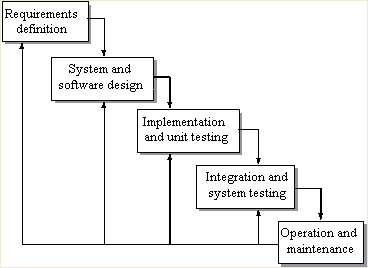
\includegraphics[width=10cm]{./iterative_waterfall_model.png}
 \caption{Iterative Waterfall Model\label{fig:iterative_waterfall_model}}
\end{figure}


\textbf{Advantages}
\begin{itemize}
\item Simple goal. Simple to understand and use. 
\item Clearly defined stages. 
\item Well understood milestones. 
\item Easy to arrange tasks. 
\item Process and results are well documented. 
\item Easy to manage. Each phase has specific deliverable and a review. 
\item Works well for projects where requirements are well understood. 
\item Works well when quality is more important than cost/schedule. 
\item Customers/End users already know about it. 
\end{itemize}


\textbf{Disadvantages}
\begin{itemize}
\item It is difficult to measure progress within stages. 
\item Cannot accommodate changing requirements. 
\item No working software is produced until late in the life cycle. 
\item Risk and uncertainty is high with this process model. 
\item Adjusting scope during the life cycle can end a project 
\item Not suitable for complex projects 
\item Not suitable for projects of long duration because in long running projects 
requirements are likely to change. 
\item Integration is done as a ''big-bang'' at the very end, which doesn't allow to identify 
any technological or business bottleneck or challenges early. 
\item Attempt to go back 2 or more phases is very costly. 
\item Percentage completion of functionality could not be determined in mid of the project 
because each functionality is undergoing some phase. 
\item Very risky, since one process can start before finishing the other. 
\end{itemize}

\section{High Level Design Document}
\subsection{Use Case Diagram}
A use case diagram presents a graphical overview of the functionality provided by a 
system in terms of actors, their goals(use cases), and any dependencies between those 
use cases. 

\begin{figure}[H]
 \centering
 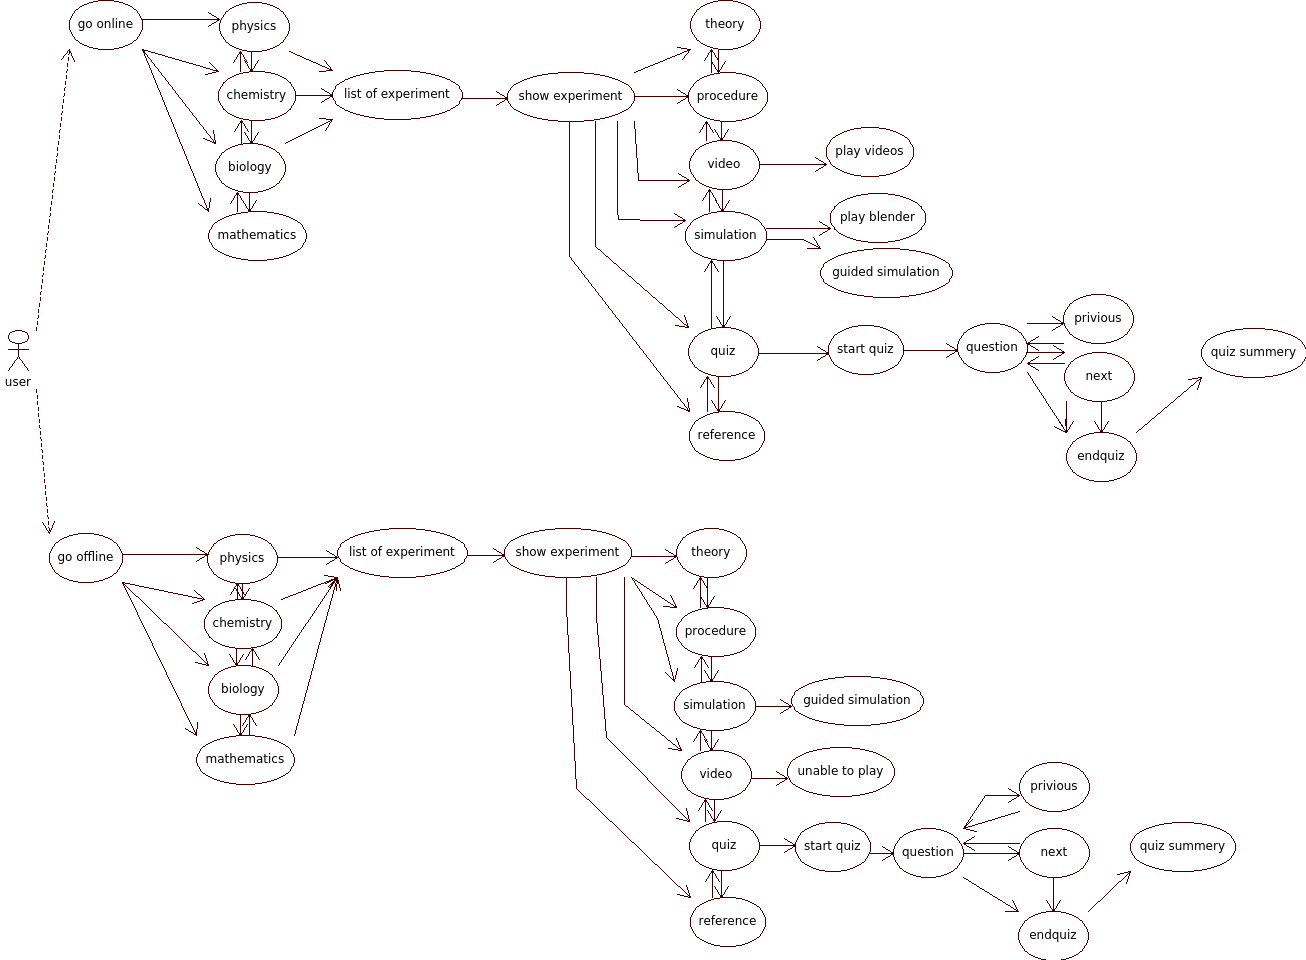
\includegraphics[width=10cm]{./usecase_app.png}
 \caption{Use Case Diagram for Android App\label{fig:usecase_app}}
\end{figure}

\pagebreak


\begin{figure}[H]
 \centering
 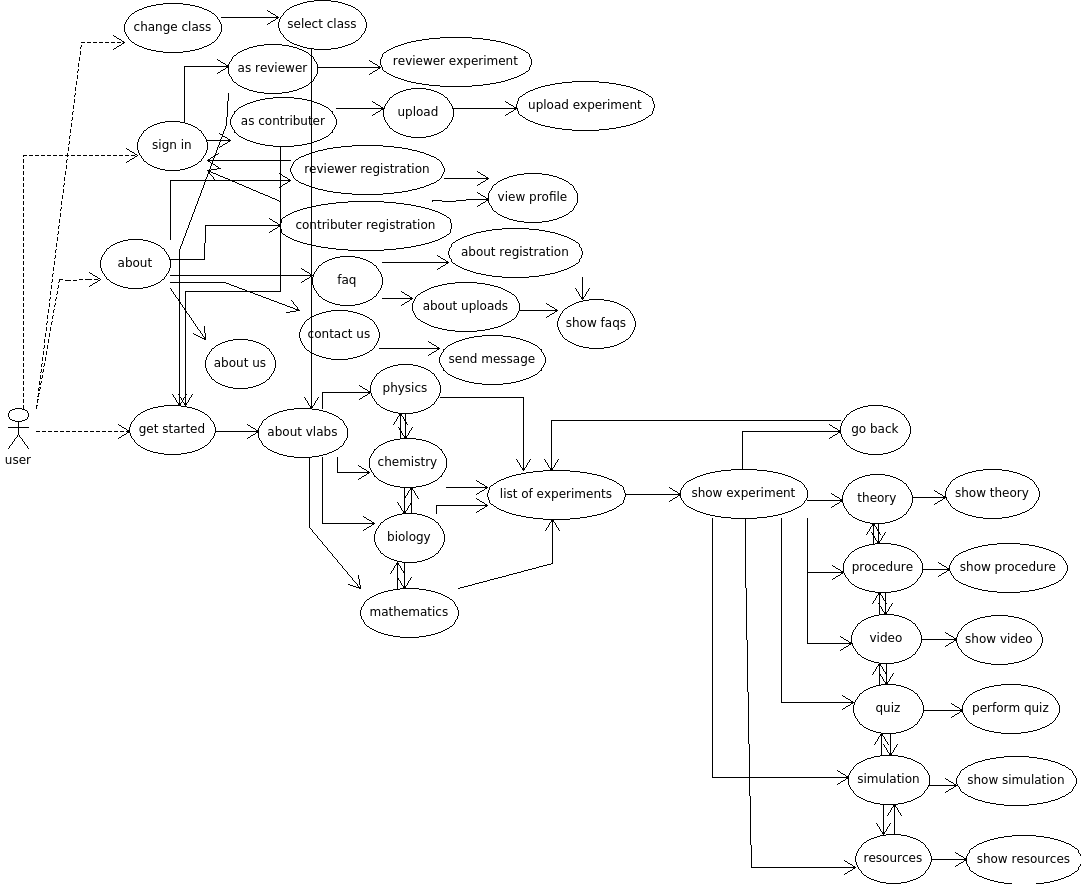
\includegraphics[width=12cm, height=16cm]{./use_case_web_new.png}
 \caption{Use Case Diagram for Web Portal\label{fig:use_case_web_new}}
\end{figure}

\pagebreak

\subsection{Use Case Description}
User is the main actor of the system. The user first launches the application and selects the 
appropriate module as required. 
\\
\\
\textbf{Go Online: }\\
Brief Description: Go Online  function enables user to enter into the Online modules of the application. \\ 
\textbf{Flow of Events:} \\
\indent  Basic Flow: User enters application with default class as 9th class. \\
\indent	Alternate Flow: User can change his class and go Online module or user enters to go Offline module.\\
Pre-condition: User opens Virtualis application with proper Internet connection.\\
Post-condition: Different modules(subject names) are displayed.\\\\
\textbf{Go Offline:}\\
Brief Description: go Offline  function enables user to enter into the saved modules of the application. \\
\textbf{Flow of Events: }\\
\indent Basic Flow: User enters application with default class as \begin{math} 9^{th} \end{math} class. \\
\indent Alternate Flow: User can change his class and go Offline module  or user enters to go Online module. \\
Pre-condition: User opens Virtualis application . \\
Post-condition: Different modules(subject names) are displayed. 
\\
\\
\textbf{Physics: }\\
Brief Description: Physics function enables user to enter into the different physics experiments of the application. \\
\textbf{Flow of Events: }\\
\indent	 Basic Flow: User enters application and tap on physics to view the physics experiments.\\
\indent	Alternate Flow: User enters application and tap on other subject.\\ 
Pre-condition: User opens Virtualis application with his class number. \\
Post-condition: Different modules(Physics experiments) are displayed. \\
\\
\textbf{Chemistry:} \\
Brief Description: Chemistry function enables user to enter into the different chemistry experiments of the application. \\
\textbf{Flow of Events: }\\
\indent	 Basic Flow: User enters application and tap on chemistry  to view the chemistry experiments. \\
\indent	Alternate Flow: User enters application and tap on other subject.\\ 
Pre-condition: User opens Virtualis application with his class number. \\
Post-condition: Different modules(Chemistry experiments) are displayed. 
\\
\\
\textbf{Biology: }\\
Brief Description: Biology function enables user to enter into the different Biology experiments of the application.\\ 
\textbf{Flow of Events: }\\
\indent	 Basic Flow: User enters application and tap on biology to view the biology experiments. \\
\indent	Alternate Flow: User enters application and tap on other subject. \\
Pre-condition: User opens Virtualis application with his class number. \\
Post-condition: Different modules(Biology experiments) are displayed. 
\\
\\
\textbf{Mathematics: }\\
Brief Description: Mathematics function enables user to enter into the different Mathematics experiments of the application. \\
\textbf{Flow of Events: }\\
\indent	  Basic Flow: User enters application and tap on mathematics to view the mathematics experiments. \\
\indent	Alternate Flow: User enters application and tap on other subject.\\ 
Pre-condition: User opens Virtualis application with his class number. \\
Post-condition: Different modules(Mathematics experiments) are displayed. 
\\
\\
\textbf{Show experiment: }\\
Brief Description: Show experiment  function enables user to enter into the different  experiment details of the application . \\
\textbf{Flow of Events: }\\
\indent	 Basic Flow: User taps on experiment name to view the experiment details.\\ 
\indent	Alternate Flow: User  tap on other subject name to view the experiments. \\
Pre-condition: User opens Virtualis application with his class number and subject name.\\ 
Post-condition: Different modules are displayed. 
\\
\\
\textbf{Theory:} \\
Brief Description: Theory function enables user to view the experiments theory module .\\ 
\textbf{Flow of Events:} \\
\indent	 Basic Flow: User taps on theory . \\
\indent	Alternate Flow: User  tap on other module. \\
Pre-condition: User opens Virtualis application and selected an experiment. \\
Post-condition: Experiment Theory is displayed. 
\\
\\
\textbf{Procedure: }\\
Brief Description: Procedure function enables user to view the experiments Procedure module . \\
\textbf{Flow of Events: }\\
\indent	 Basic Flow: User taps on procedure . \\
\indent	Alternate Flow: User  tap on other module. \\
Pre-condition: User opens Virtualis application and selected an experiment.\\ 
Post-condition: Experiment Procedure is displayed.\\ 
\\
\\
\textbf{Video: }\\
Brief Description: Video  function enables user to view the experiments Video module.\\
\textbf{Flow of Events:} \\
\indent	 Basic Flow: User taps on video . \\
\indent	Alternate Flow: User  tap on other module. \\
Pre-condition: User opens Virtualis application and selected an experiment.\\ 
Post-condition: Experiment Videos are displayed. 
\\
\\
\textbf{Simulation: }\\
Brief Description: Simulation function enables user to view the experiments simulation module . \\
\textbf{Flow of Events: } \\
\indent	 Basic Flow: User taps on simulation . \\
\indent	Alternate Flow: User  tap on other module. \\
Pre-condition: User opens Virtualis application and selected an experiment. \\
Post-condition: Experiments simulations are displayed. 
\\
\\
\textbf{Quiz: }
Brief Description: Quiz function enables user to practice the experiments quiz module . \\
\textbf{Flow of Events: }\\
\indent	 Basic Flow: User taps on quiz. \\
\indent	Alternate Flow: User  tap on other module. \\
Pre-condition: User opens Virtualis application and selected an experiment. \\
Post-condition: Experiments related questions are displayed. 
\\
\\
\textbf{Resources: }
Brief Description: Resources function enables user to view the experiments Resources . \\
\textbf{Flow of Events: }\\
\indent	 Basic Flow: User taps on resources . \\
\indent	Alternate Flow: User  tap on other module. \\
Pre-condition: User opens Virtualis application and selected an experiment. \\
Post-condition: Experiment Resources are displayed. 
\\
\\
\textbf{Run Blender: }
Brief Description: Run Blender  function enables user to  view the experiments simulation in Blender Player . \\
\textbf{Flow of Events: }\\
\indent	 Basic Flow: User taps on run Blender . \\
\indent	Alternate Flow: User  tap on guided simulation. \\
Pre-condition: User opens Virtualis application and selected simulation module. \\
Post-condition: Experiments Blender simulation is played.
\\
\\
\textbf{Guided simulation: }
Brief Description: Guided simulation function enables user to  view the experiments simulation in Android Application . \\
\textbf{Flow of Events: }\\
\indent	 Basic Flow: User  tap on guided simulation . \\
\indent	Alternate Flow:  User taps on run Blender .\\
Pre-condition: User opens Virtualis application and selected simulation module.\\ 
Post-condition: Experiments simulation is shown to perform experiment.\\

\pagebreak

\subsection{Activity Diagram}

Activity diagrams are graphical representations of work flows of step-wise activities 
and actions with support for choice, iteration and concurrency. An activity diagram 
shows the overall flow of control. 

%  ~\ref{fig:iterative_waterfall_model} 
\begin{figure}[H]
 \centering
 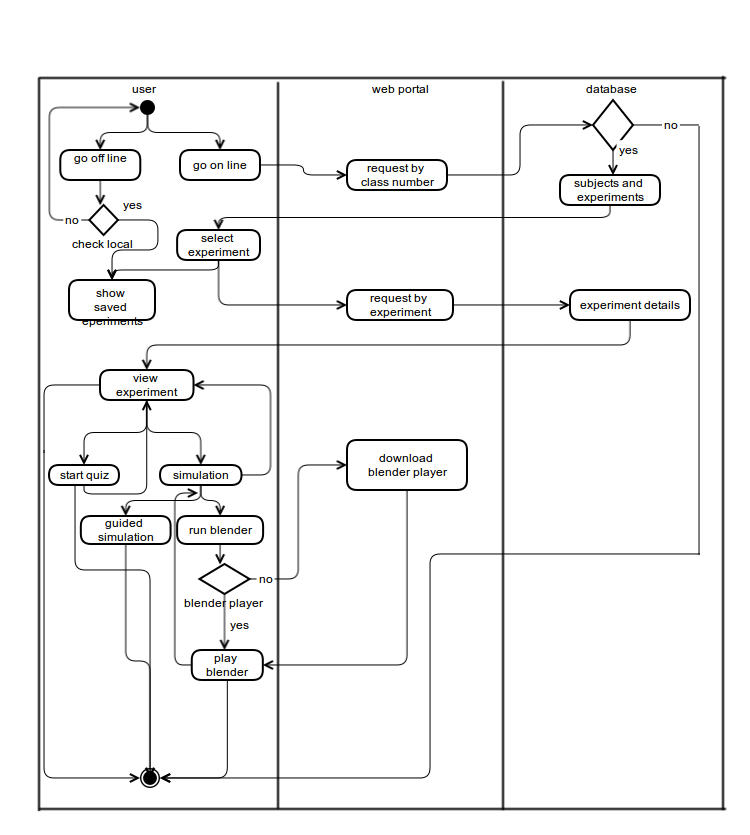
\includegraphics[width=15cm]{./activity.png}
 \caption{Activity Diagram\label{fig:activity}}
\end{figure}

\pagebreak

\subsection{Class Diagram}
Activity diagrams are graphical representations of work flows of step-wise activities 
and actions with support for choice, iteration and concurrency. An activity diagram 
shows the overall flow of control.\\
 
 %  ~\ref{fig:iterative_waterfall_model} 
\begin{figure}[H]
 \centering
 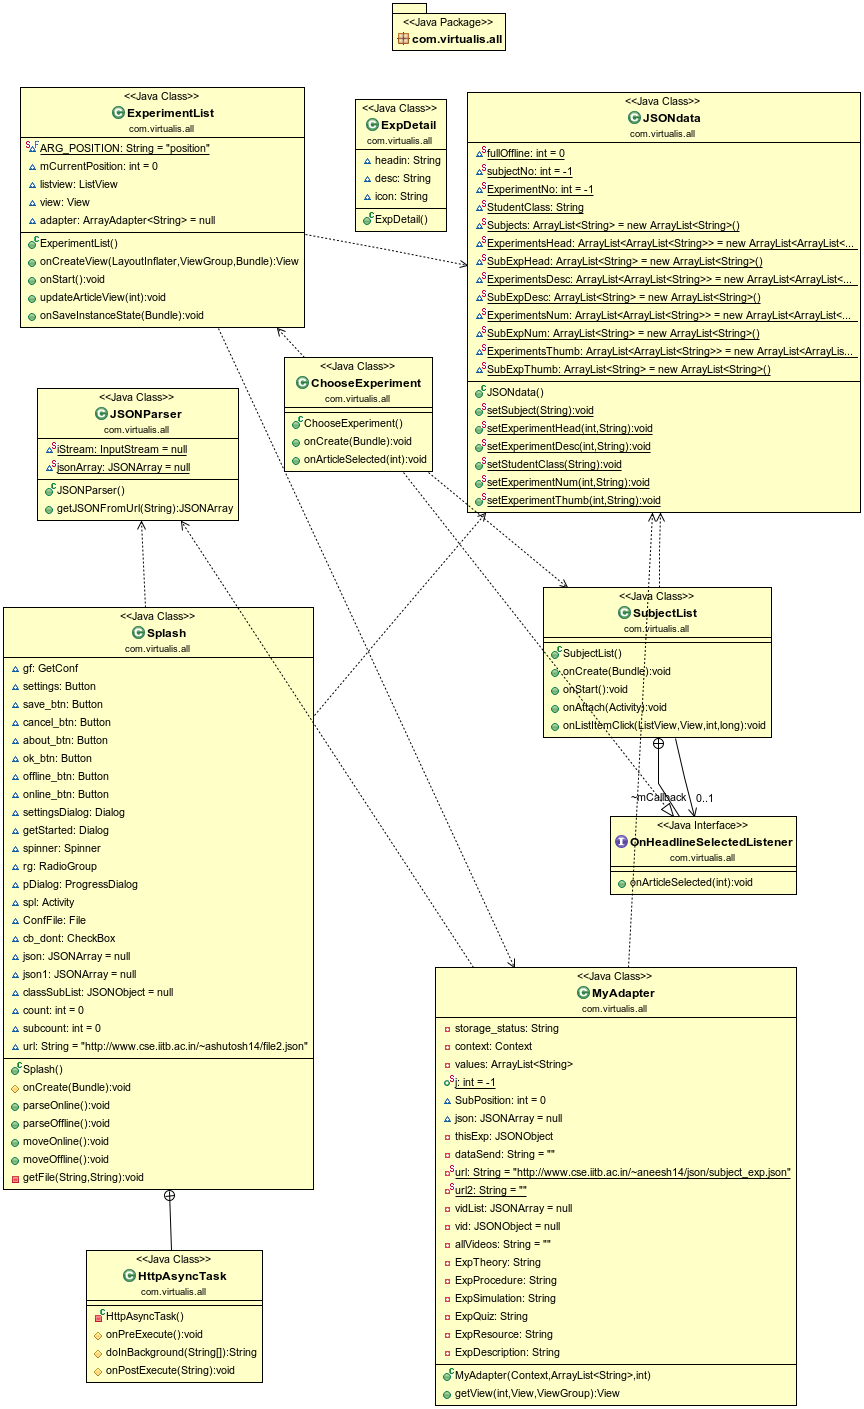
\includegraphics[width=10cm]{./class_all.png}
 \caption{Class Diagram\label{fig:class_all}}
\end{figure}

%  ~\ref{fig:iterative_waterfall_model} 
\begin{figure}[H]
 \centering
 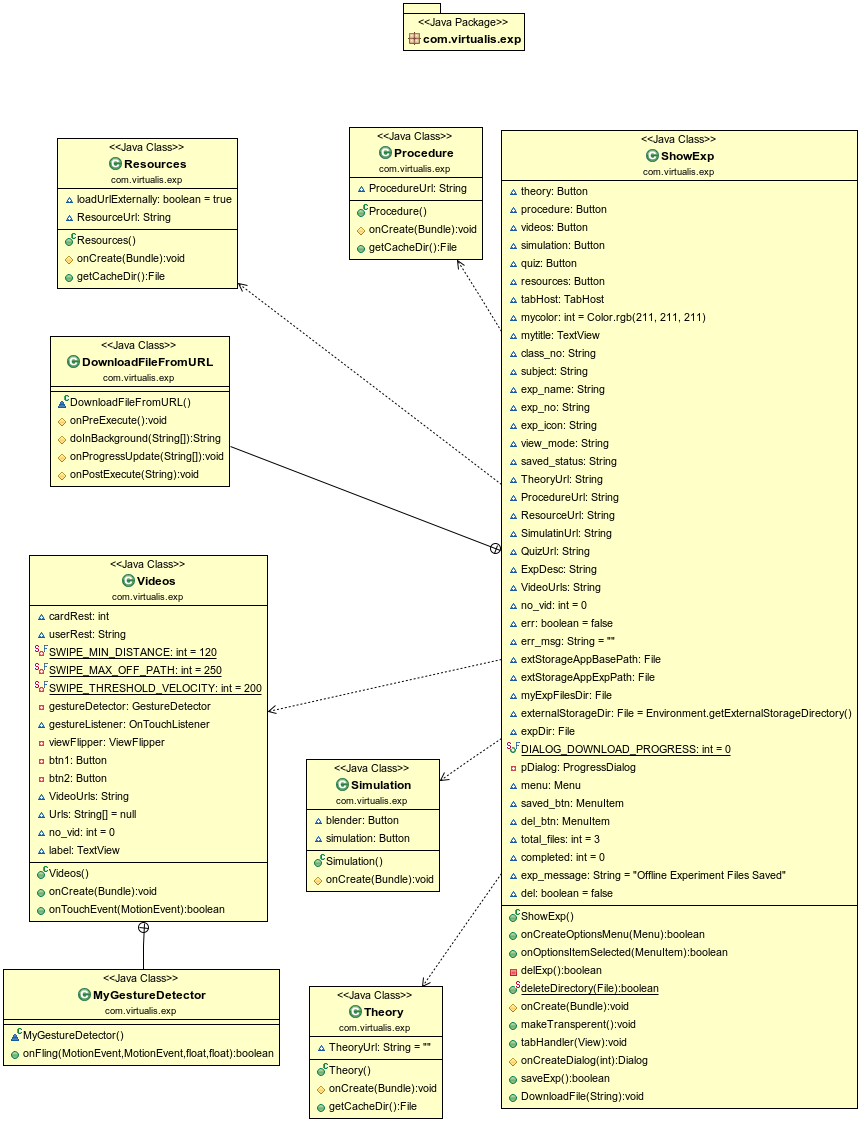
\includegraphics[width=10cm]{./class_exp.png}
 \caption{Experiment Class Diagram\label{fig:class_exp}}
\end{figure}

%  ~\ref{fig:iterative_waterfall_model} 
\begin{figure}[H]
 \centering
 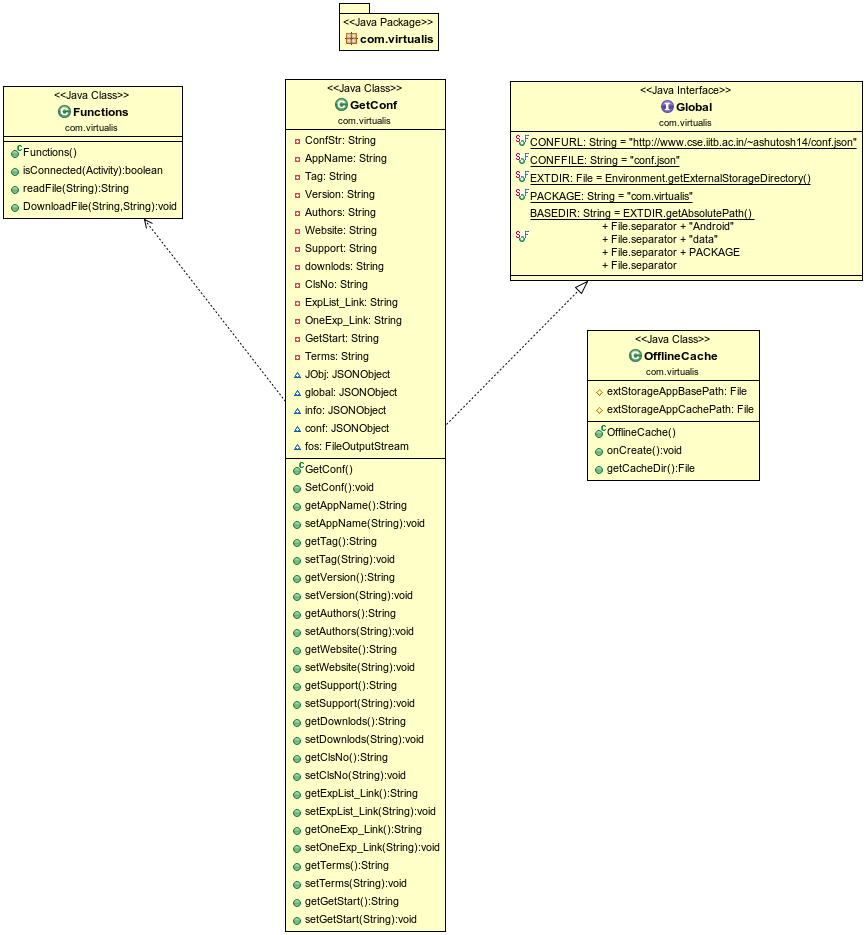
\includegraphics[width=10cm]{./class_main.png}
 \caption{Main Class Diagram\label{fig:class_main}}
\end{figure}

%  ~\ref{fig:iterative_waterfall_model} 
\begin{figure}[H]
 \centering
 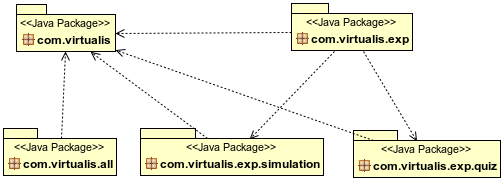
\includegraphics[width=10cm]{./class_package.png}
 \caption{Package Class Diagram\label{fig:class_package}}
\end{figure}

%  ~\ref{fig:iterative_waterfall_model} 
\begin{figure}[H]
 \centering
 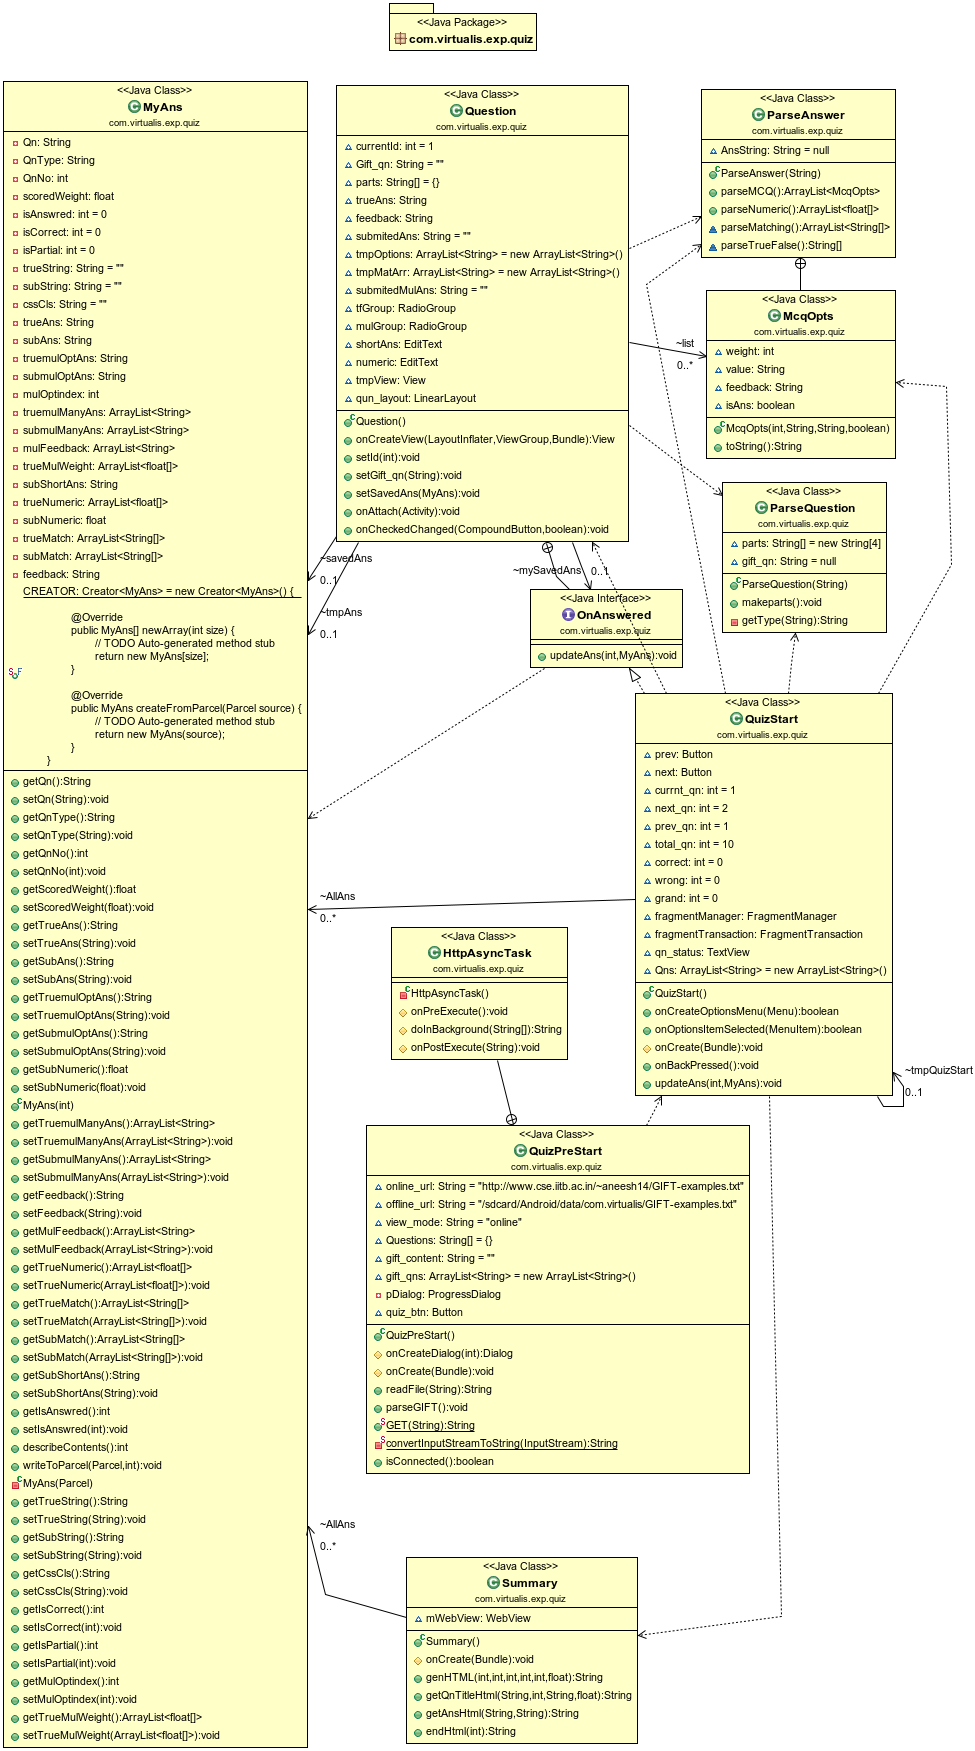
\includegraphics[width=10cm]{./class_quiz.png}
 \caption{Quiz Class Diagram\label{fig:class_quiz}}
\end{figure}

%  ~\ref{fig:iterative_waterfall_model} 
\begin{figure}[H]
 \centering
 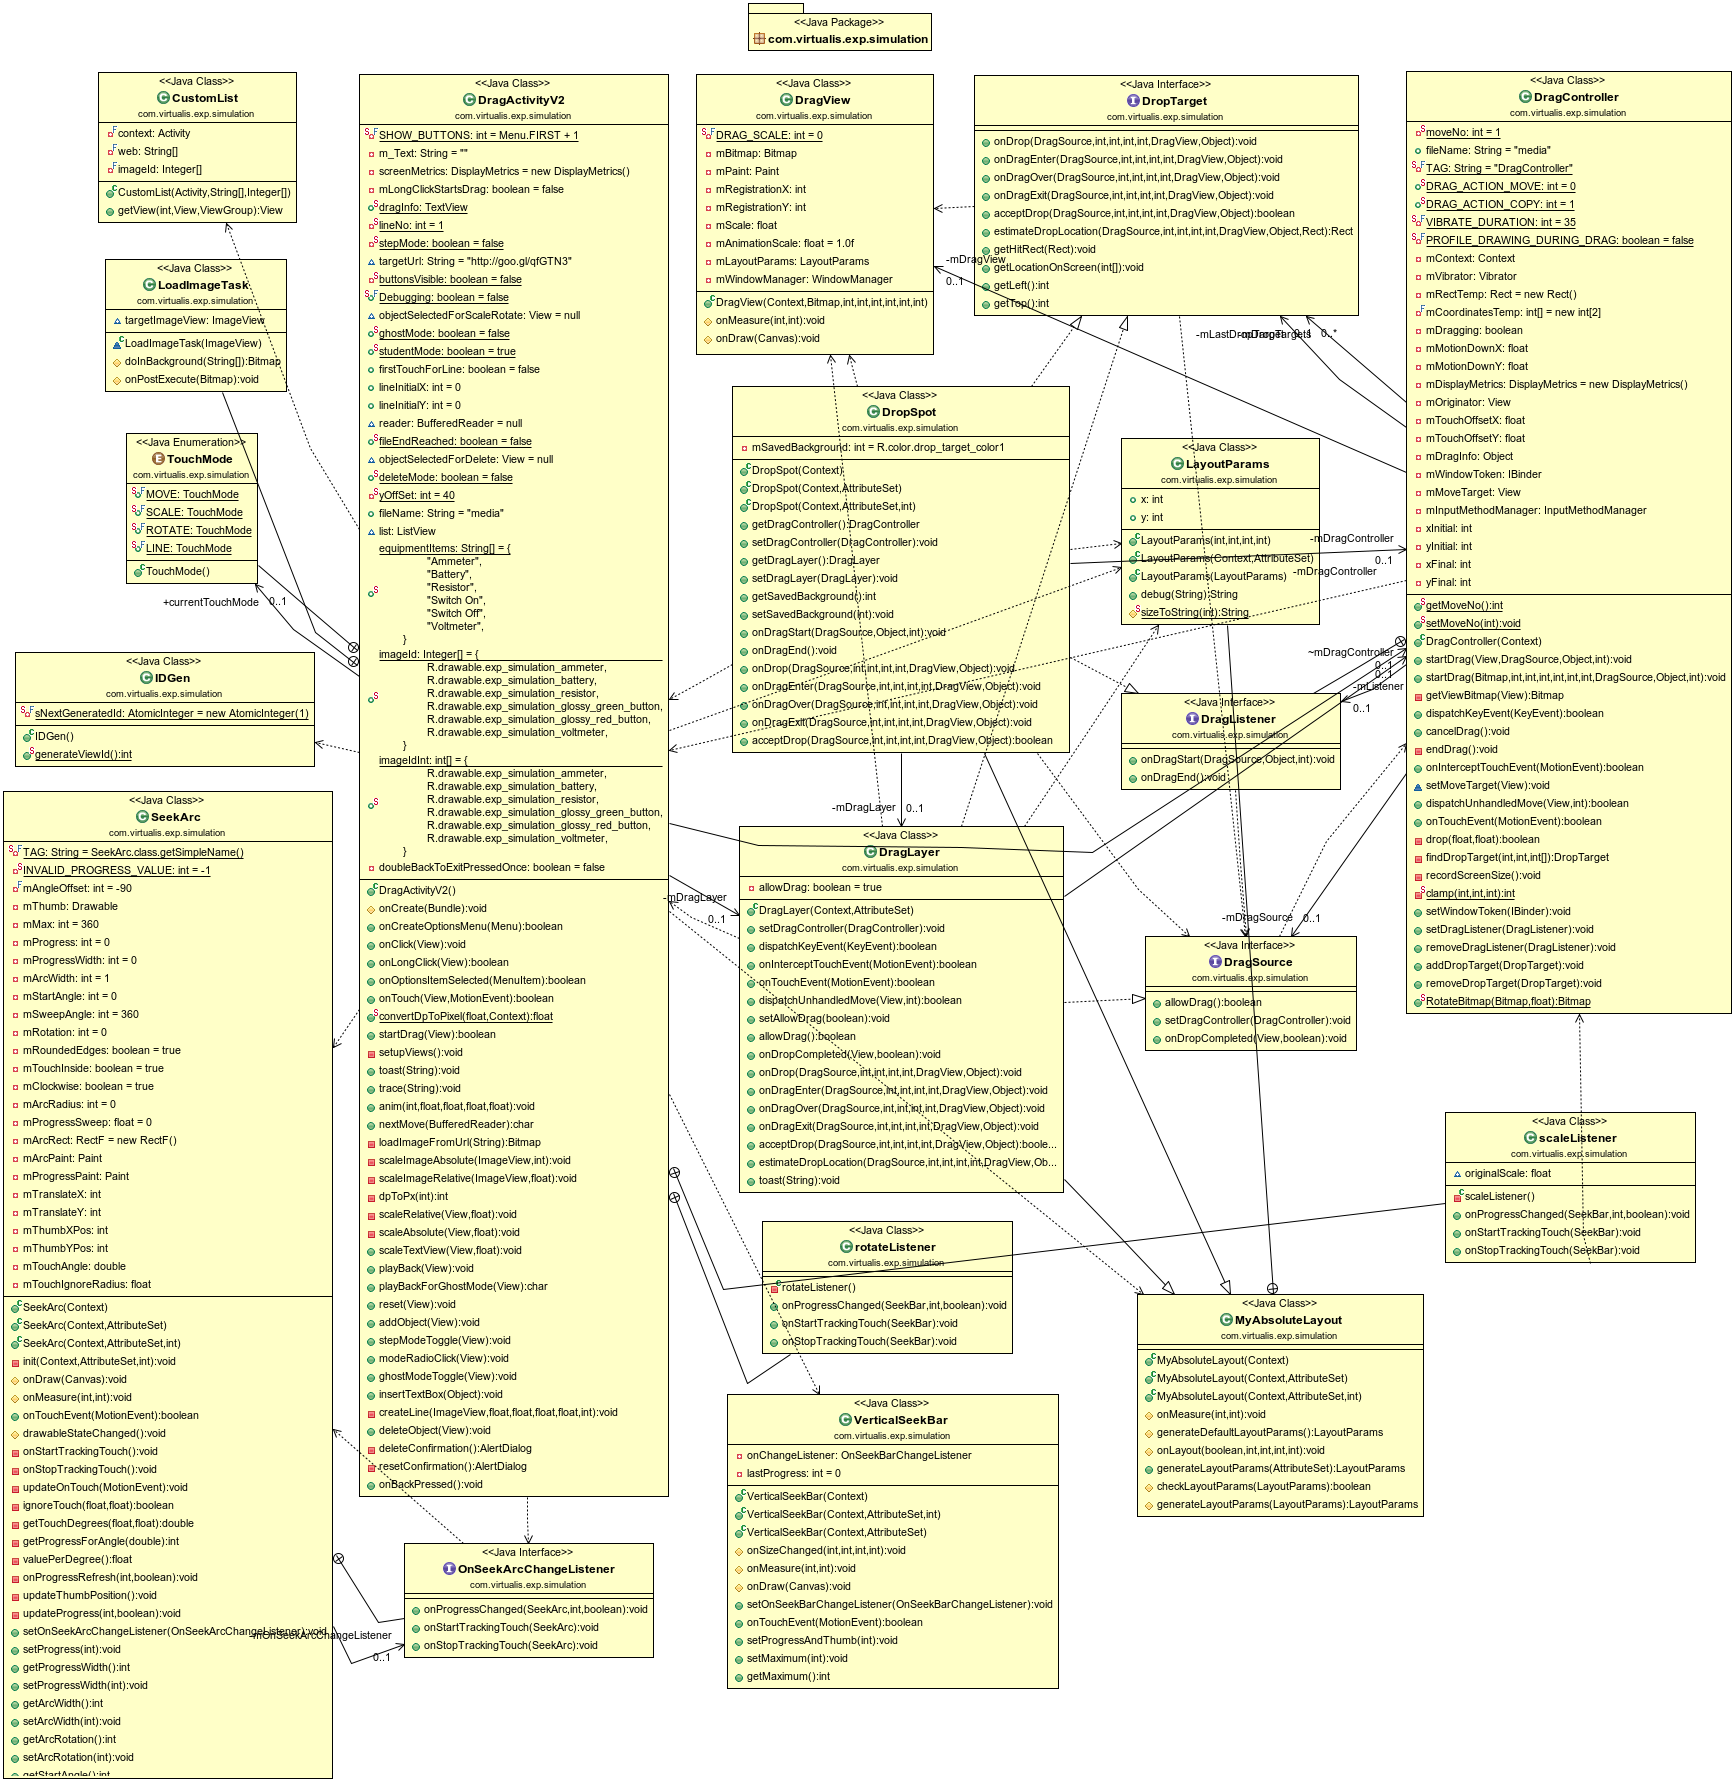
\includegraphics[width=10cm]{./class_simulation.png}
 \caption{Simulation Class Diagram\label{fig:class_simulation}}
\end{figure}

\subsection{Data Flow Diagrams}

%  ~\ref{fig:iterative_waterfall_model} 
\begin{figure}[H]
 \centering
 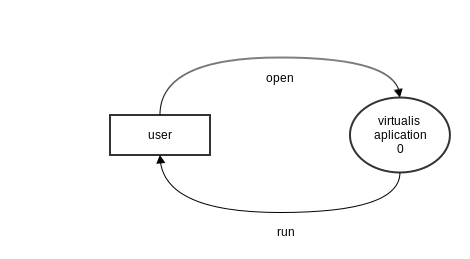
\includegraphics[width=10cm]{./dfd_level0.png}
 \caption{DFD Level 0\label{fig:dfd_level0}}
\end{figure}

%  ~\ref{fig:iterative_waterfall_model} 
\begin{figure}[H]
 \centering
 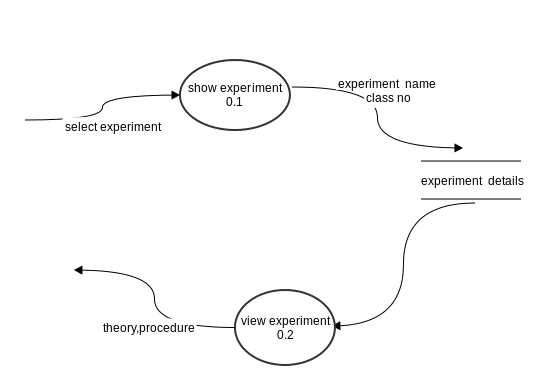
\includegraphics[width=10cm]{./dfd_level1_image1.png}
 \caption{DFD Level 1\label{fig:dfd_level1_image1}}
\end{figure}

%  ~\ref{fig:iterative_waterfall_model} 
\begin{figure}[H]
 \centering
 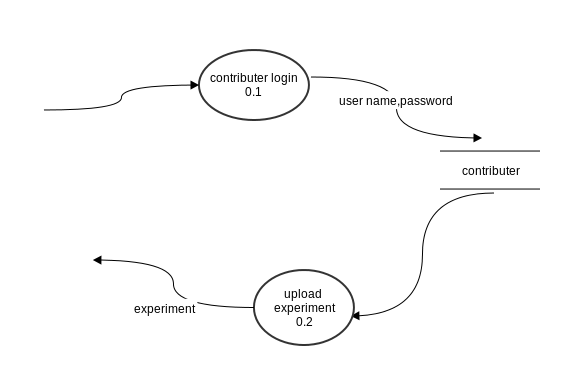
\includegraphics[width=10cm]{./dfd_level1_image2.png}
 \caption{DFD Level 1\label{fig:dfd_level1_image2}}
\end{figure}

\subsection{Sequence Diagram:}

%  ~\ref{fig:iterative_waterfall_model} 
\begin{figure}[H]
 \centering
 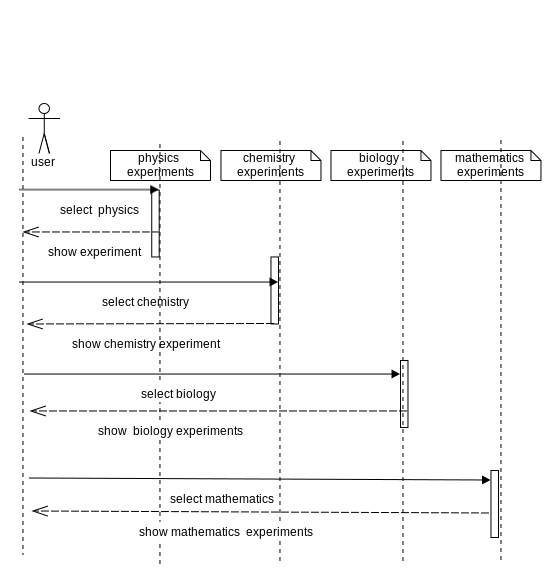
\includegraphics[width=10cm]{./sequence_1.png}
 \caption{Sequence Diagram\label{fig:sequence_1}}
\end{figure}

%  ~\ref{fig:iterative_waterfall_model} 
\begin{figure}[H]
 \centering
 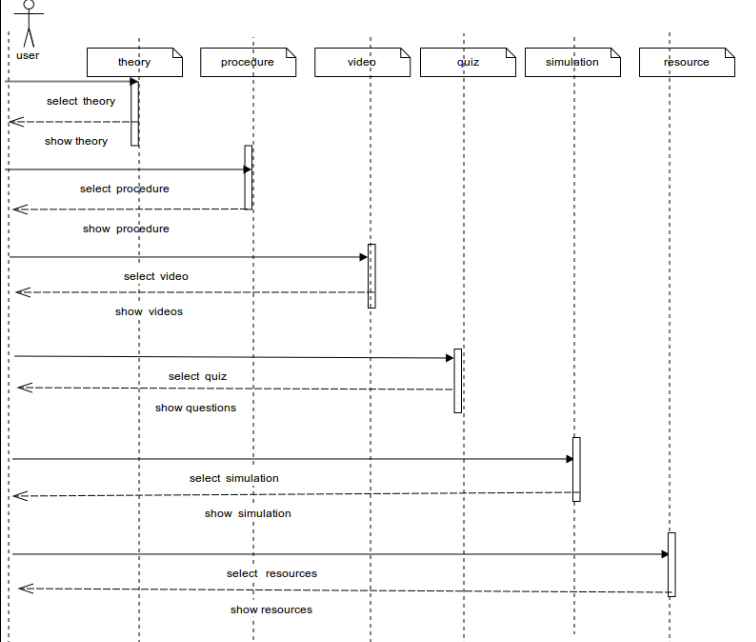
\includegraphics[width=10cm]{./sequence_2.png}
 \caption{Sequence Diagram\label{fig:sequence_2}}
\end{figure}

\subsection{E-R Diagram :}

%  ~\ref{fig:iterative_waterfall_model} 
\begin{figure}[H]
 \centering
 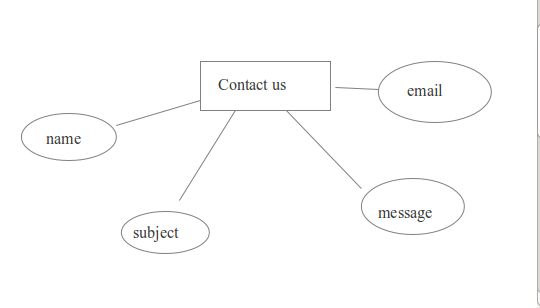
\includegraphics[width=10cm]{./er_contact.png}
 \caption{Contact ER Diagram\label{fig:er_contact}}
\end{figure}

%  ~\ref{fig:iterative_waterfall_model} 
\begin{figure}[H]
 \centering
 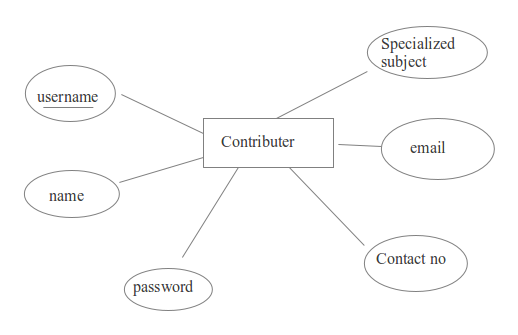
\includegraphics[width=10cm]{./er_contributer.png}
 \caption{Contributor ER Diagram\label{fig:er_contributer}}
\end{figure}

%  ~\ref{fig:iterative_waterfall_model} 
\begin{figure}[H]
 \centering
 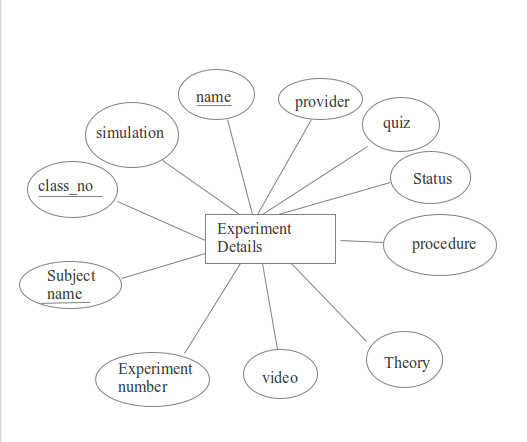
\includegraphics[width=10cm]{./er_experiment.png}
 \caption{Experiment ER Diagram\label{fig:er_experiment}}
\end{figure}

%  ~\ref{fig:iterative_waterfall_model} 
\begin{figure}[H]
 \centering
 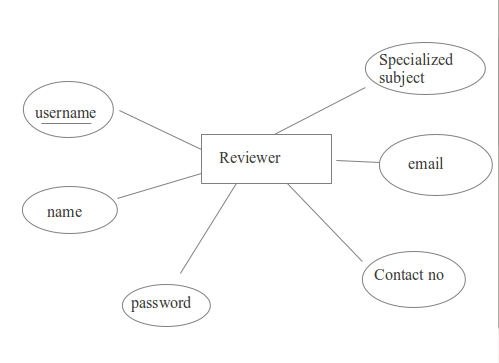
\includegraphics[width=10cm]{./er_reviewer.png}
 \caption{Reviewer ER Diagram\label{fig:er_reviewer}}
\end{figure}

\chapter{Testing}
Software testing is an investigation conducted to provide information about the quality of the 
product or service under test. Software testing also provides an objective, independent view 
of the software to allow the business to appreciate and understand the risks at implementation 
of the software. Test technique includes the process of executing a program or application 
with the intent of finding software bugs. 
Software testing can be stated as the process of verifying and validating that a software 
program/application/product: 

\begin{itemize}
\item Meet the requirements that guide its design and development
\item Work as expected
\item Can be deployed with the same characteristics.
\end{itemize}

Software testing can be implemented at any time depending on the testing method employed 
in the development process. However, most of the test effort traditionally occurs after the 
requirements have been defined and the coding process has been completed. It is observed 
that fixing a bug is less expensive if found earlier in the development process. Although in 
the agile approaches most of the test effort is, conversely, on-going. As such, the 
methodology of the test is governed by the software development methodology adopted. 
\section{Testing technique used}
Several testing techniques have been performed on the system such as unit testing, 
integration testing and system testing. 
\subsection{Unit Testing: }
Unit testing, also known as component testing refers to tests that verify the 
functionality of a specific section of code, usually at the function level. Unit 
testing is a software development process that involves synchronized 
application of a broad spectrum of defect prevention and detection strategies 
in order to reduce software development risks, time, and costs. 
\subsection{Integration Testing }
The purpose of integration testing is to verify functional, performance, and 
reliability requirements placed on major design items. Integration testing is 
any type of software testing that seeks to verify the interfaces between 
components against a software design. Integration testing works to expose 
defects in the interfaces and interaction between integrated components 
(modules). 
\\
\\
\textbf{Black-box testing}- It is a method of software testing that examines the 
functionality of an application(e.g. what the software does) without 
peering into its internal structures or workings. 
\\
\\
\textbf{White-box testing} - It is a method of testing software that tests internal 
structures or workings of an application, as opposed to its 
functionality. In white-box testing an internal perspective of the 
system, as well as programming skills, are used to design test cases. 
In this testing, we performed Boundary Value Analysis. 

\subsection{System Testing}
System testing tests a completely integrated system to verify that it meets its 
requirements. In addition, the software testing should ensure that the program, 
as well as working as expected, does not also destroy or partially corrupt its 
operating environment or cause other processes within that environment to 
become inoperative. 
\\
\\
System testing of software or hardware is testing conducted on a complete, 
integrated system to evaluate the system's compliance with its specified 
requirements. System testing falls within the scope of black box testing, and as 
such, should require no knowledge of the inner design of the code or logic. In this testing we performed Alpha testing. 

\chapter{User Manual - Virtualis}


\section{Introduction}
Virtualis v0.1 is an Android App, created to provide android interface of accessing the virtual lab experiments. Here student can read all the theory, procedure, resources, watch the videos, take the quiz that is associated with the give experiment and finally he can also follow the guided simulation or Blender simulation. He can access the contents in two modes 

\begin{itemize}
\item Online Mode
\item Offline Mode
\item Online - Offline Mode
\end{itemize}

\section{Online Mode}
The online mode can be opened if there is a proper net connectivity. In Online mode the user can view list of subjects along with the list of experiments of that subject\\
Saved experiments and unsaved experiments are differentiated by View saved button appearing at experiment name

\begin{itemize}

\item If user selects the saved experiment the application goes to offline mode and shows the saved experiment

\item If user selects unsaved experiment the application opens the experiment in online mode

\item Once the user selects an experiment he is able to view the theory , procedure, video, quiz,simulation and resources of the Experiment by clicking on respective modules

\end{itemize}
\pagebreak

\subsection{Function for Experiment}
Users is provided with below options to work with a Experiment for offline mode
\begin{itemize}
\item Save Experiment
\item Update Experiment
\item Delete Experiment
\end{itemize}

\subsubsection{Save Experiment}
Here, user can save the current experiment for offline view mode

\subsubsection{Update Experiment}
Here, user can Update the current experiment which is already saved for offline view mode

\subsubsection{Delete Experiment}
Here, user can Delete the current experiment which is already saved for offline view mode


\subsection{Parts of an Experiment}
One Experiment is divided into various parts that are namely
\begin{itemize}
\item Theory
\item Procedure
\item Videos
\item Simulation
\item Quiz
\item Resources
\end{itemize}

\subsubsection{Theory}
This section displays the theory related to selected experiment

\subsubsection{Procedure}
This section displays the procedure related to selected experiment

\subsubsection{videos}
This section plays the different videos that are provided for a selected experiment

\subsubsection{Simulation}
This section provide two modes of simulation for a selected experiment
\begin{itemize}
\item Run Guided Simulation
\item Open Blender Simulation
\end{itemize}

\subsubsection{Run Guided Simulation}

This module guide the student to follow the steps that followed by the teacher while doing the experiment in the android platform. It includes 

\begin{itemize}
\item Addition of Object
\item Rotation of Object
\item Scaling of Object
\item Drawing the new Object
\end{itemize}

\subsubsection{Run Blender}

This module plays the interactive animation of that experiment if the Blender player is installed in that device else it asks user to download and install the Blender player.

\subsubsection{Quiz}
This section displays the procedure related to selected experiment\\
Quiz module having next and previous buttons to switch between the questions quiz module having submit quiz button to submit the quiz .once he submitted then the summery report of his performance will be displayed through which he can evaluate himself.\\
It includes
\begin{itemize}
\item Displaying the Question
\item Walk through around all the question
\item Summary of the all the questions
\end{itemize}

\subsubsection{Resources}
This section displays the extra resources related to selected experiment

\pagebreak

\section{Offline Mode}

In offline mode the previously saved experiments are shown to user. The user views list of subjects along with the list of saved experiments of that subject once the user selects an experiment he is able to view the theory , procedure, video, simulation and resources of the Experiment by clicking on respective modules


\section{Online - Offline Mode}

Online - Offline mode, is similar to Online Mode the difference is he can switch from Online to Offline that's why this mode is named like that, this can be done by clicking the ''view saved exp'' button in the list of experiment, then he can view the previously saved experiments are shown to user in like Online Mode. The user views list of subjects along with the list of saved experiments of that subject once the user selects an experiment he is able to view the theory , procedure, video, simulation and resources of the Experiment by clicking on respective modules




\section{Flow of Virtualis}
\begin{figure}[H]
 \centering
 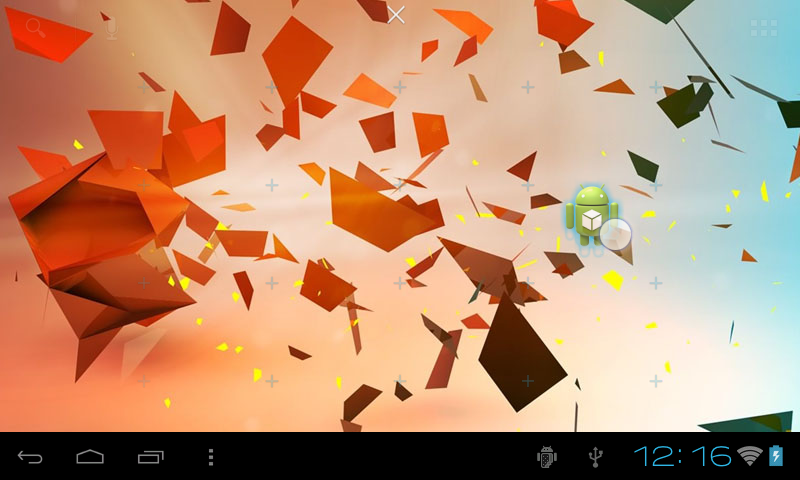
\includegraphics[width=15cm]{./1.png}
 \caption{Open Virtualis\label{fig:1}}
\end{figure}

\pagebreak
\begin{figure}[H]
 \centering
 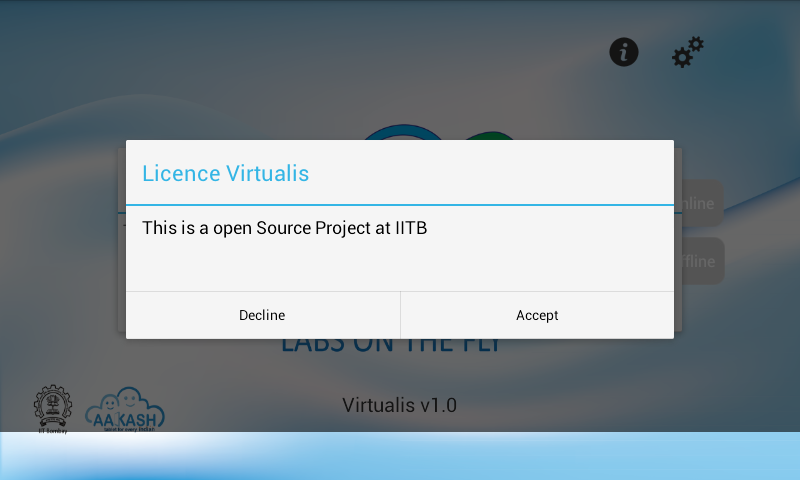
\includegraphics[width=15cm]{./2.png}
 \caption{Accept The License\label{fig:2}}
\end{figure}

\begin{figure}[H]
 \centering
 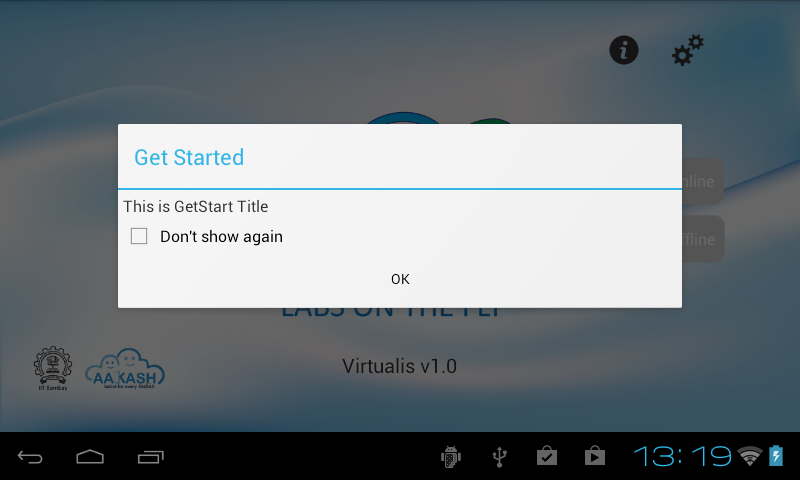
\includegraphics[width=15cm]{./3.png}
 \caption{Get Started \label{fig:3}}
\end{figure}

\begin{figure}[H]
 \centering
 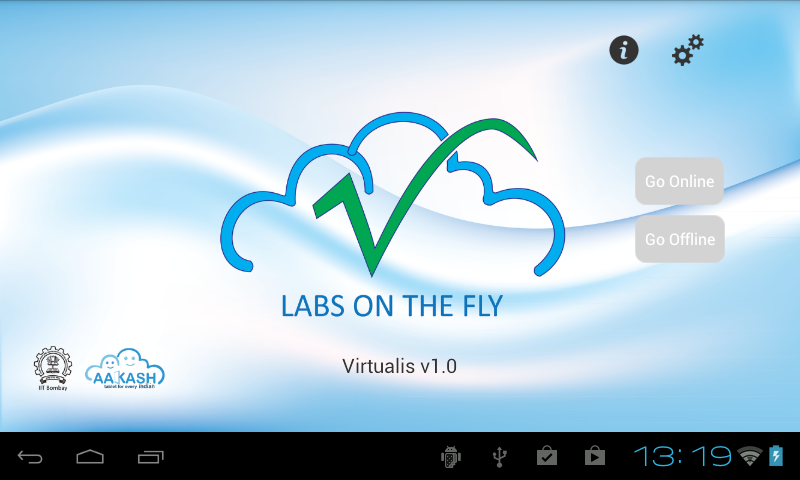
\includegraphics[width=15cm]{./4.png}
 \caption{Virtualis Splash Screen\label{fig:4}}
\end{figure}

\begin{figure}[H]
 \centering
 
\includegraphics[width=15cm]{./5.png}
 \caption{About us Button\label{fig:5}}
\end{figure}

\begin{figure}[H]
 \centering
 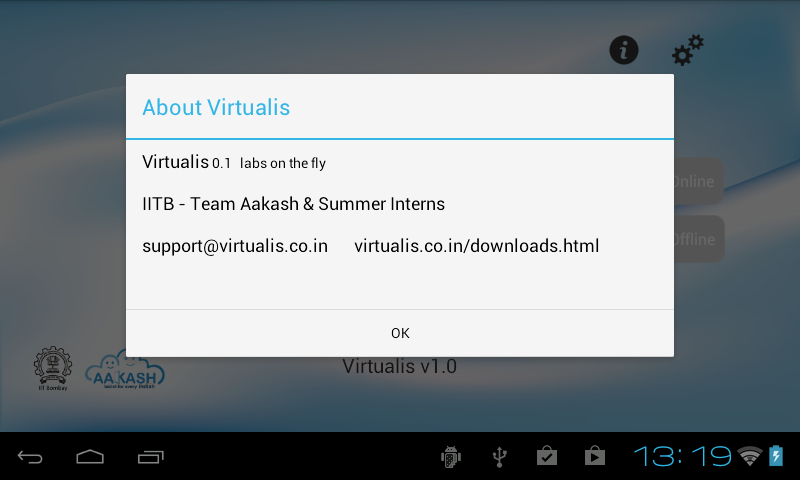
\includegraphics[width=15cm]{./6.png}
 \caption{About us\label{fig:6}}
\end{figure}

\begin{figure}[H]
 \centering
 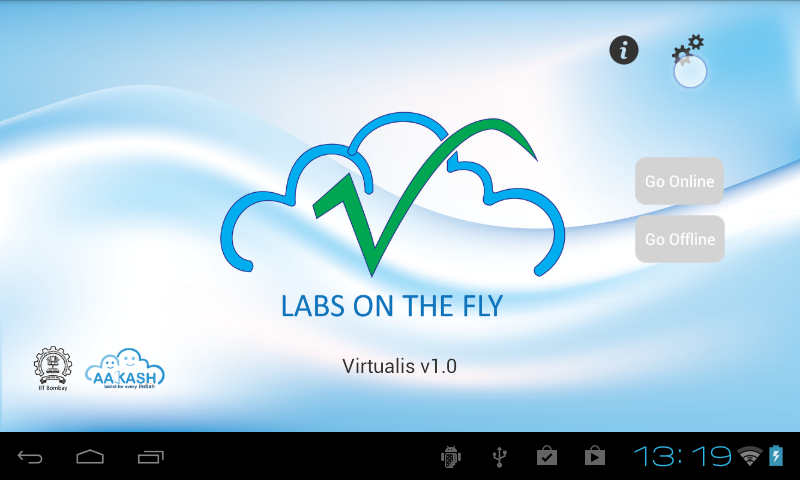
\includegraphics[width=15cm]{./7.png}
 \caption{Settings \label{fig:7}}
\end{figure}

\begin{figure}[H]
 \centering
 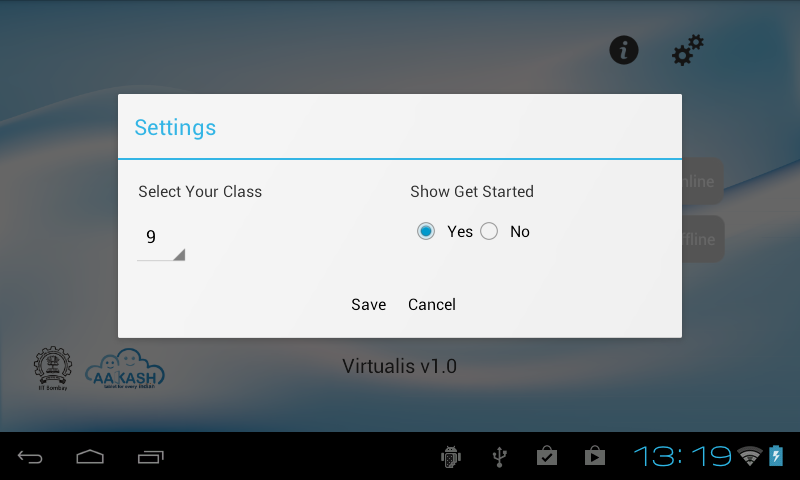
\includegraphics[width=15cm]{./8.png}
 \caption{Settings \label{fig:8}}
\end{figure}

\begin{figure}[H]
 \centering
 
\includegraphics[width=15cm]{./11.png}
 \caption{Go Online\label{fig:11}}
\end{figure}

\begin{figure}[H]
 \centering
 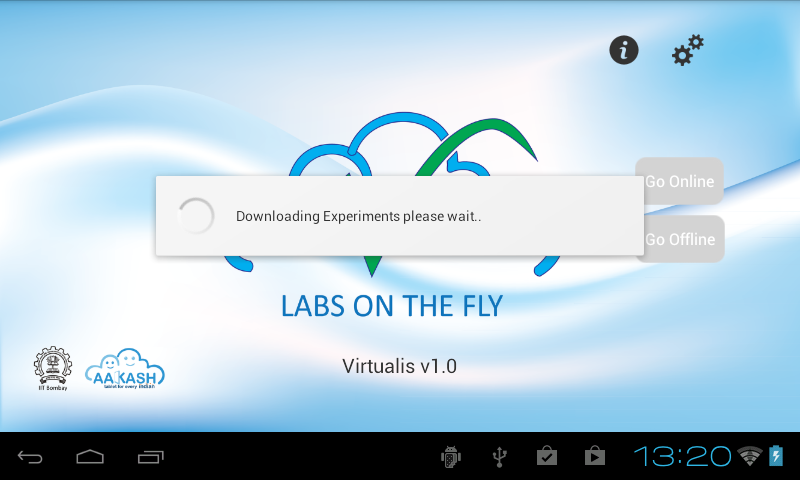
\includegraphics[width=15cm]{./12.png}
 \caption{Downloading Experiments\label{fig:12}}
\end{figure}

\begin{figure}[H]
 \centering
 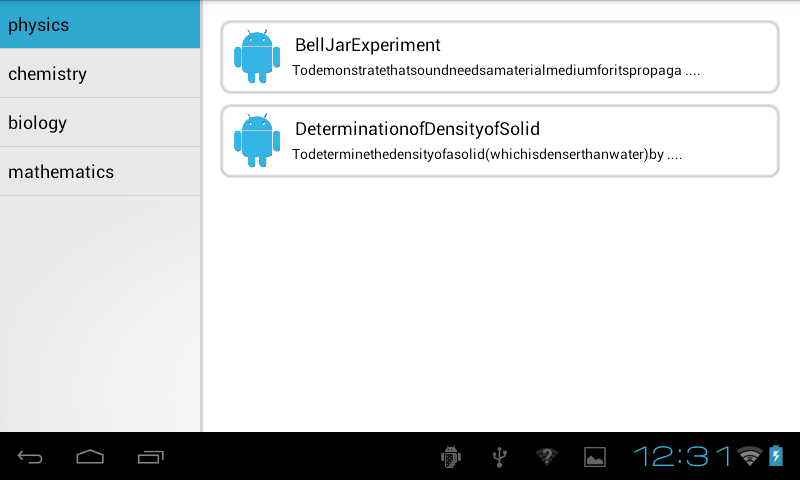
\includegraphics[width=15cm]{./13.png}
 \caption{List of Experiments and Subjects \label{fig:13}}
\end{figure}

\begin{figure}[H]
 \centering
 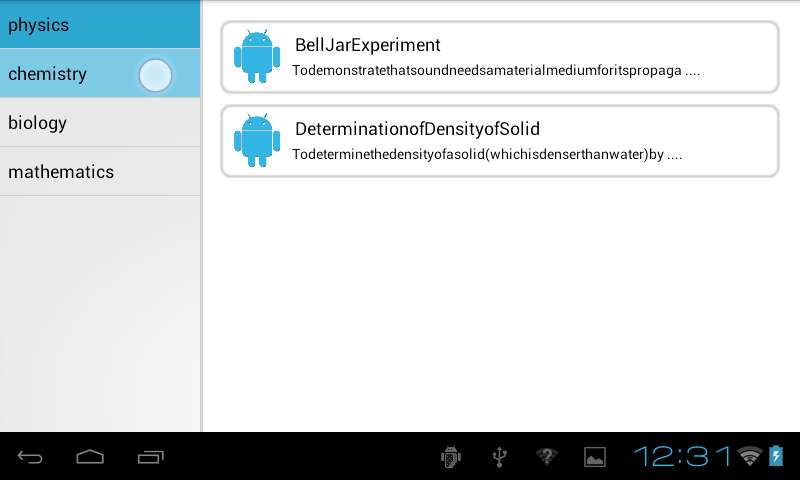
\includegraphics[width=15cm]{./14.png}
 \caption{Select subject\label{fig:14}}
\end{figure}

\begin{figure}[H]
 \centering
 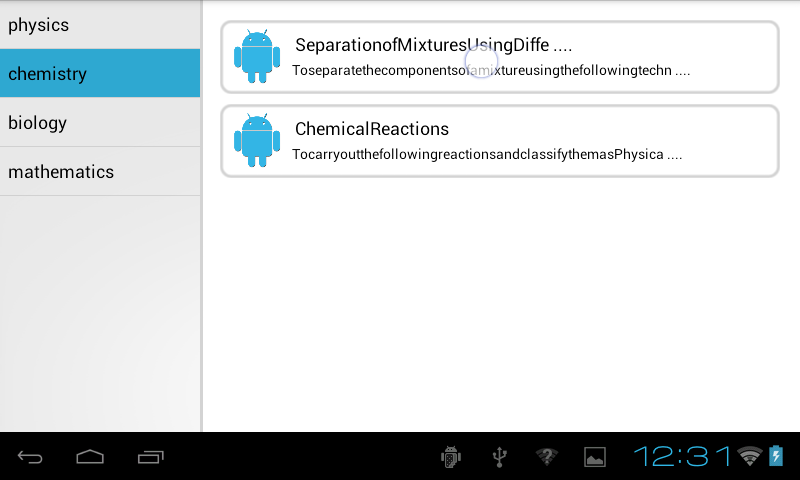
\includegraphics[width=15cm]{./16.png}
 \caption{Select experiment\label{fig:16}}
\end{figure}


\begin{figure}[H]
 \centering
 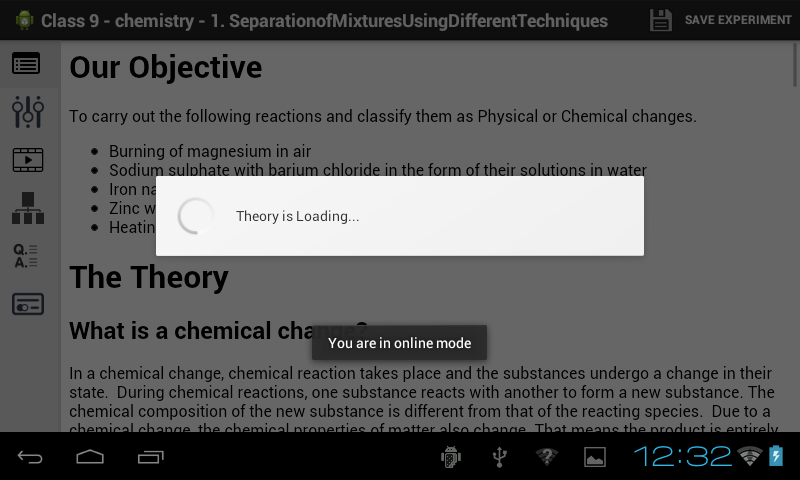
\includegraphics[width=15cm]{./17.png}
 \caption{Theory Loading\label{fig:17}}
\end{figure}


\begin{figure}[H]
 \centering
 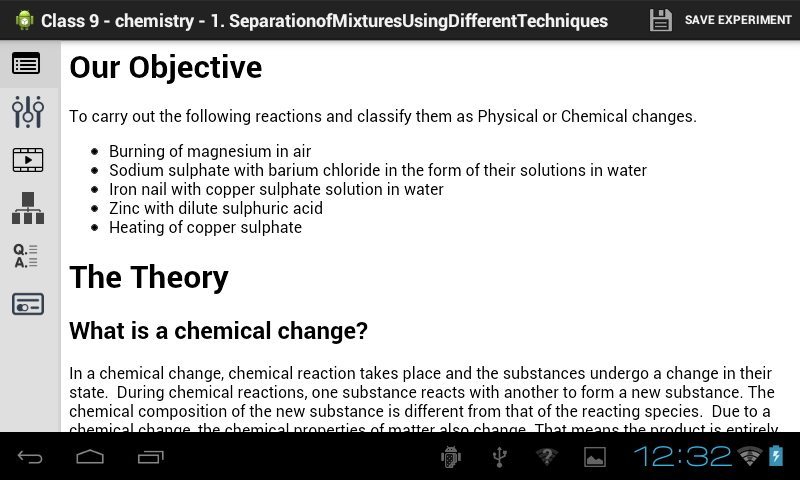
\includegraphics[width=15cm]{./18.png}
 \caption{Experiment Theory \label{fig:18}}
\end{figure}

\begin{figure}[H]
 \centering
 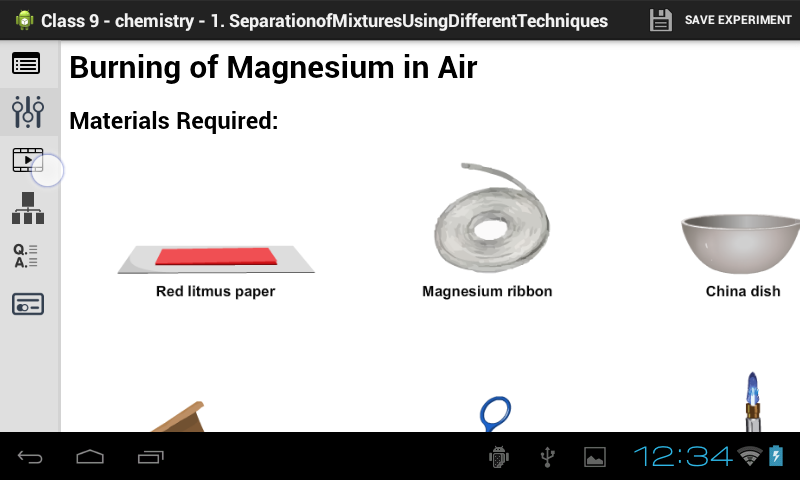
\includegraphics[width=15cm]{./20.png}
 \caption{Procedure \label{fig:20}}
\end{figure}

\begin{figure}[H]
 \centering
 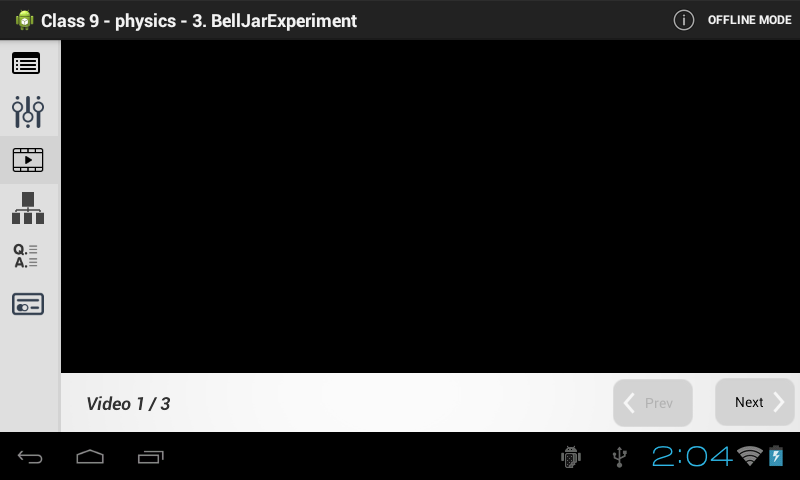
\includegraphics[width=15cm]{./22.png}
 \caption{Videos \label{fig:22}}
\end{figure}



\begin{figure}[H]
 \centering
 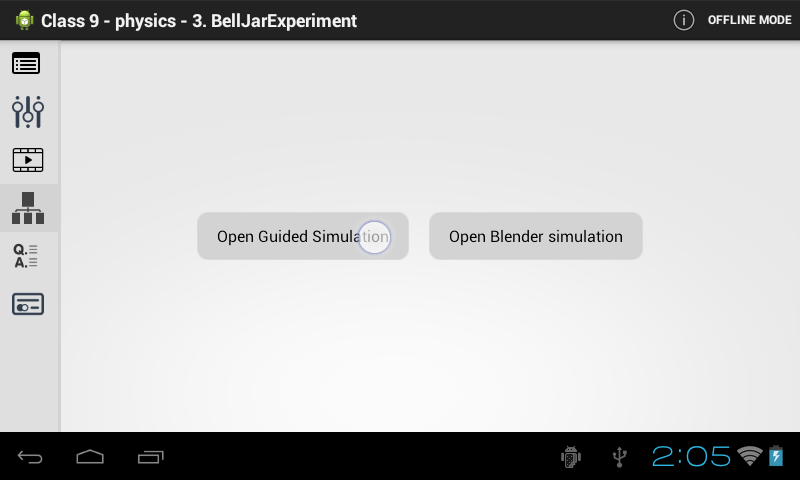
\includegraphics[width=15cm]{./24.png}
 \caption{Open Guided Simulation \label{fig:24}}
\end{figure}

\begin{figure}[H]
 \centering
 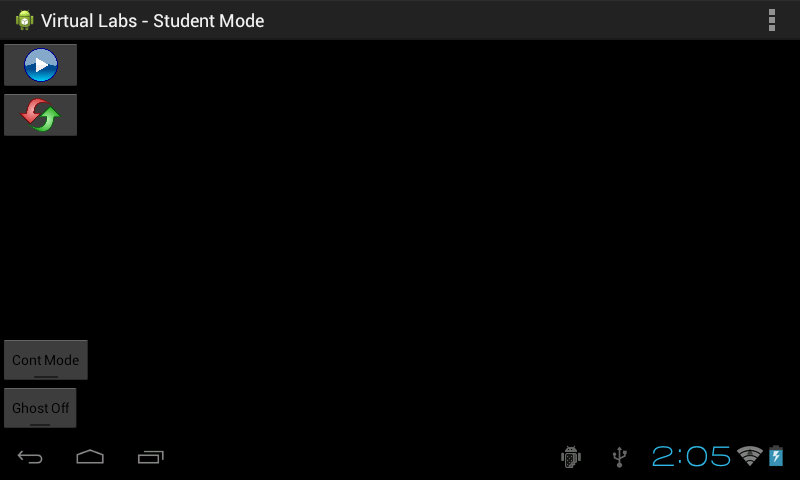
\includegraphics[width=15cm]{./25.png}
 \caption{Guided Simulation Portal \label{fig:25}}
\end{figure}



\begin{figure}[H]
 \centering
 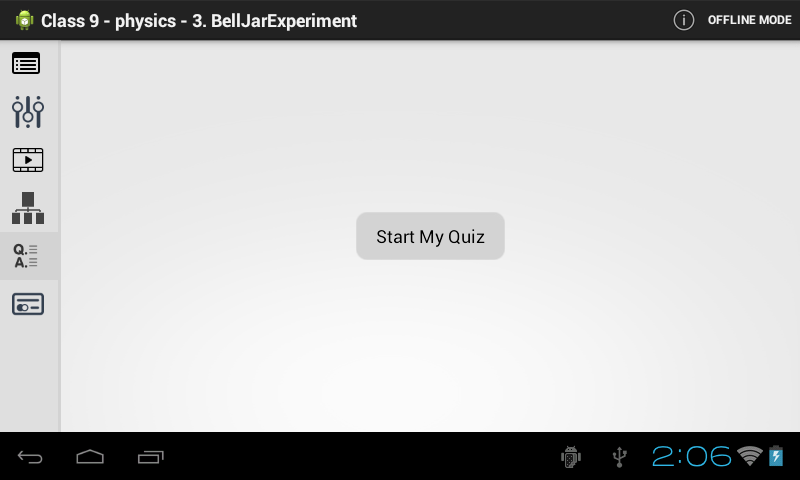
\includegraphics[width=15cm]{./27.png}
 \caption{Start My Quiz \label{fig:27}}
\end{figure}

\begin{figure}[H]
 \centering
 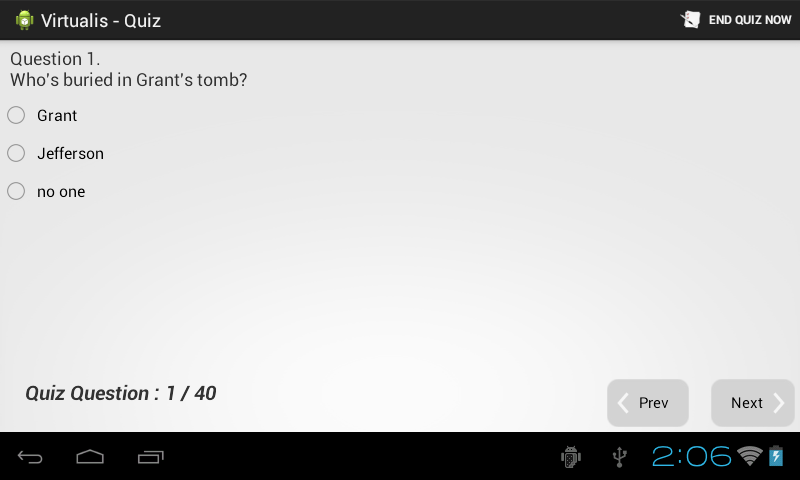
\includegraphics[width=15cm]{./28.png}
 \caption{Displaying Question\label{fig:28}}
\end{figure}

\begin{figure}[H]
 \centering
 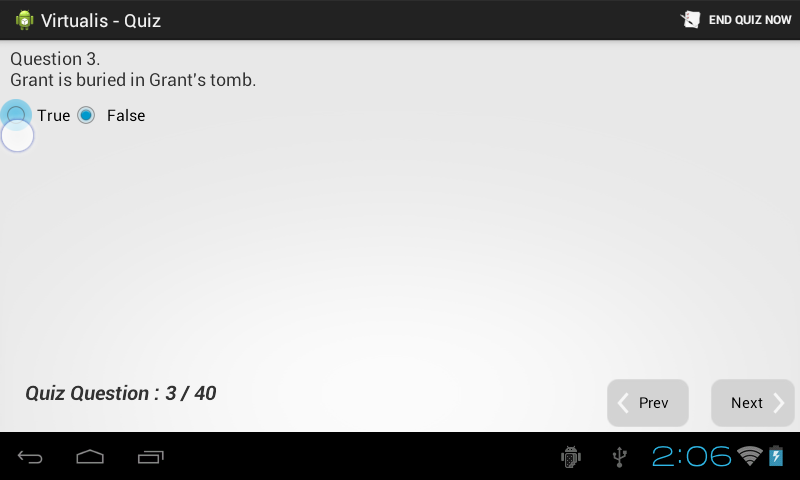
\includegraphics[width=15cm]{./29.png}
 \caption{Answering Questions \label{fig:29}}
\end{figure}

\begin{figure}[H]
 \centering
 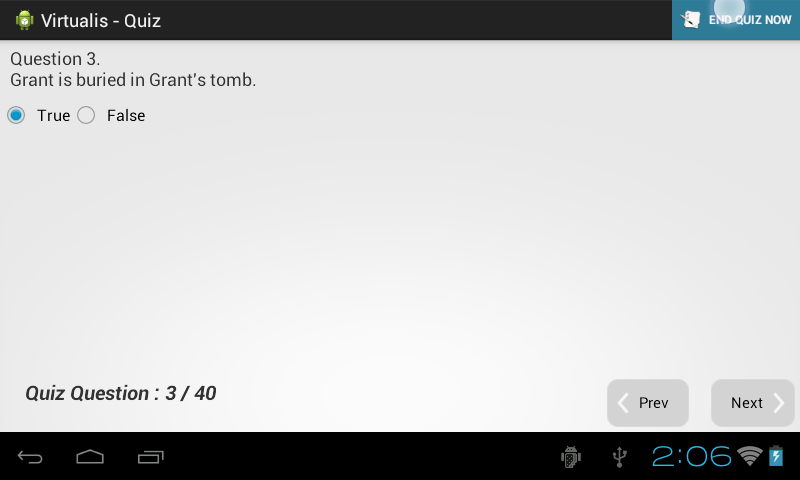
\includegraphics[width=15cm]{./30.png}
 \caption{Submit Quiz \label{fig:30}}
\end{figure}

\begin{figure}[H]
 \centering
 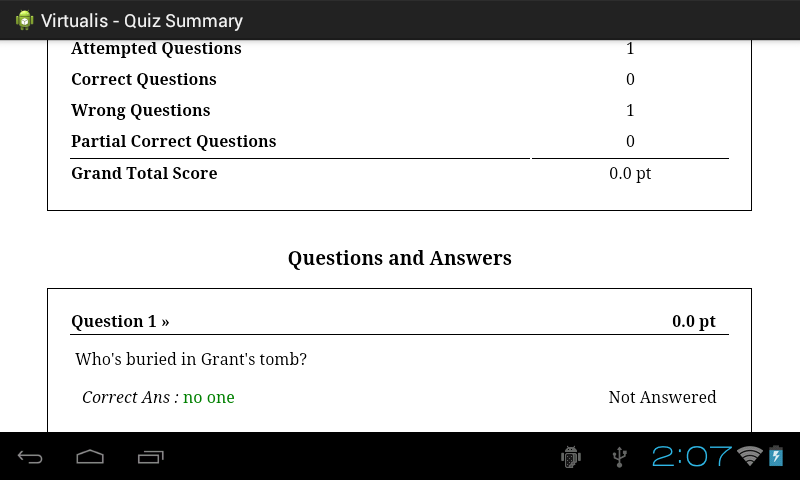
\includegraphics[width=15cm]{./31.png}
 \caption{Summary of Quiz\label{fig:31}}
\end{figure}

\begin{figure}[H]
 \centering
 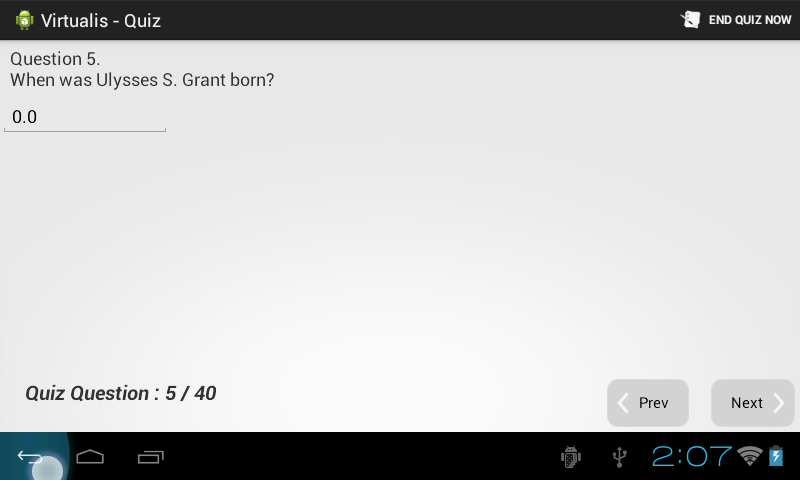
\includegraphics[width=15cm]{./32.png}
 \caption{Go Back \label{fig:32}}
\end{figure}

\begin{figure}[H]
 \centering
 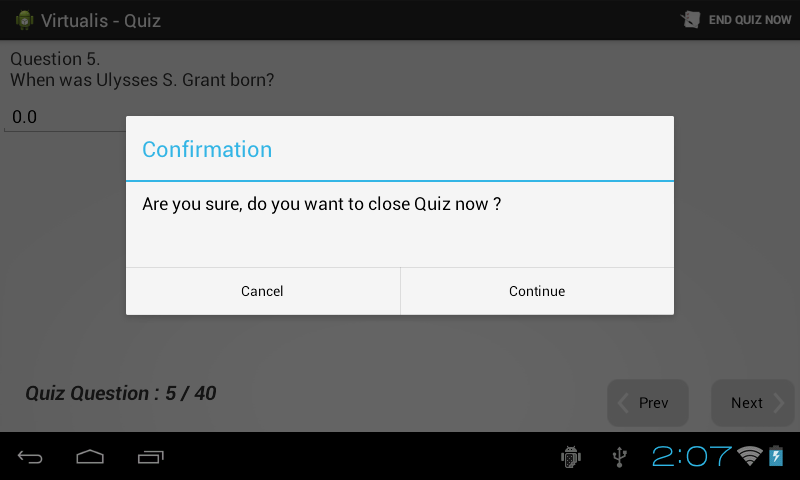
\includegraphics[width=15cm]{./33.png}
 \caption{Confirm Quiz Close\label{fig:33}}
\end{figure}


\begin{figure}[H]
 \centering
 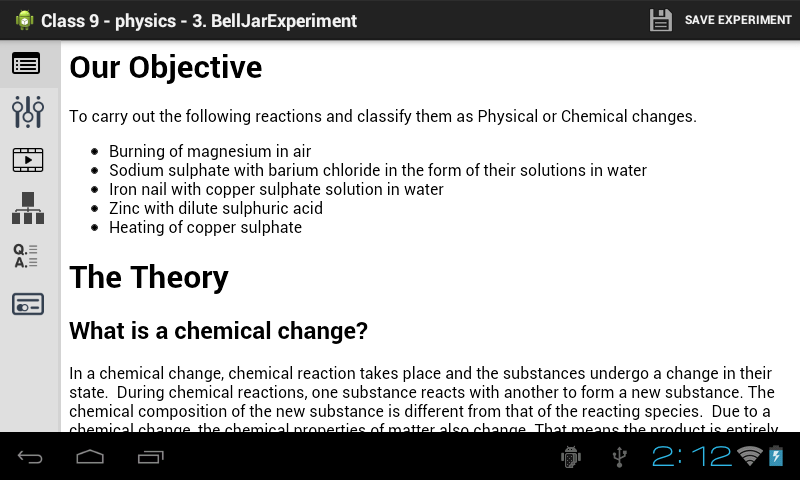
\includegraphics[width=15cm]{./37.png}
 \caption{Save Experiment\label{fig:37}}
\end{figure}

\begin{figure}[H]
 \centering
 \includegraphics[width=15cm]{./34.png}
 \caption{Update Experiment \label{fig:34}}
\end{figure}

\begin{figure}[H]
 \centering
 \includegraphics[width=15cm]{./35.png}
 \caption{Delete Experiment\label{fig:35}}
\end{figure}

\begin{figure}[H]
 \centering
 \includegraphics[width=15cm]{./36.png}
 \caption{Confirm Delete Experiment \label{fig:36}}
\end{figure}

\begin{figure}[H]
 \centering
 \includegraphics[width=15cm]{./38.png}
 \caption{Go Offline Mode\label{fig:38}}
\end{figure}


\begin{figure}[H]
 \centering
 \includegraphics[width=15cm]{./37_1.png}
 \caption{View Saved Exp - Online Offline Navigation \label{fig:37_1}}
\end{figure}



\begin{figure}[H]
 \centering
 \includegraphics[width=15cm]{./40.png}
 \caption{App in Offline View Mode\label{fig:40}}
\end{figure}

\pagebreak

\section{Simulation Flow View}

There are 2 Modes in which the whole application can be used in :
\begin{itemize}
\item Play Mode 
\item Ghost Mode 
\end{itemize}
Play Mode :  
The play mode has further 2 modes :  
\begin{itemize}
\item Step Mode 
\item Continuous Mode 
\end{itemize}

\subsection{Continuous Mode :}
Continuous Mode will play the whole experiment animation in one go whereas the Step Mode will 
play the experiment step by step for the user to understand it carefully. 


\subsection{Ghost Mode :}
The Ghost mode is the mode in which the student performs the experiment along with a guide. 
The guiding images will be transparent and will show the student what the next move is 
supposed to be and the student will have to perform that move.\\
\\
There is a correction mechanism also , i.e. If the student doesn't perform the right move the 
animation will not proceed forward and will wait till the student performs the right move with an 
error margin of 10\%. 
\\
The modes in Ghost Mode are :  
\begin{itemize}
\item Move Mode
\item Scale/ Rotate Mode
\item Delete Mode
\end{itemize}

\subsubsection{Move Mode :}
The student can select an object and perform a translational movement by simple drag and drop 
and the application will guide him and also correct him. 

\subsubsection{Scale/ Rotate Mode :}
In the scale and rotate mode the student can scale and rotate the selected object and proceed with the experiment. 

\subsubsection{Delete Mode :} 
In the delete mode the student can delete the selected object from the screen. \\


\subsubsection{Play Button} 
The play button performs a variety of functions 

\begin{itemize}
\item If the application is in Continuous Mode ­ It will play the whole animation/experiment in one go.
\item If the application is in Step Mode ­ It will play the experiment in step by step manner on every click
\item If the application is in the Ghost Mode ­ It will start the guided mode for the student to follow and perform the experiment.
\end{itemize}

\subsubsection{Reset Button :}

It resets the whole experiment/application to its default state and then one can start over. There 
is a confirmation pop­up for the reset button in case the student touched it unintentionally. 

\subsubsection{The GhostMode Toggle:}

This toggle Button toggles the ghost Mode of the application.
\subsubsection{The Cont/Step Mode Toggle:}

This toggle button toggles the Step/Continuous Mode of the application

\subsubsection{Mode Group :} 

This appears only when the ghost mode is selected and is used to switch between the different 
touch modes.

\subsubsection{The scale and Rotate bar :}
These bars appear only when the Scale/Rotate mode is selected.

\begin{figure}[H]
 \centering
 \includegraphics[width=15cm]{./101.png}
 \caption{The starting screen of the simulation part of the Application.\label{fig:101}}
\end{figure}

\begin{figure}[H]
 \centering
 \includegraphics[width=15cm]{./102.png}
 \caption{To play the whole animation click the following Play Button ­ Note the Mode Button shows Cont Mode ­ i.e. Continuous Mode
\label{fig:102}}
\end{figure}

\begin{figure}[H]
 \centering
 \includegraphics[width=15cm]{./103.png}
 \caption{To reset the whole simulation/experiment ­ Touch the Reset Button\label{fig:103}}
\end{figure}

\begin{figure}[H]
 \centering
 \includegraphics[width=15cm]{./104.png}
 \caption{Confirmation Prompt for reset \label{fig:104}}
\end{figure}

\begin{figure}[H]
 \centering
 \includegraphics[width=15cm]{./106.png}
 \caption{For changing the mode from Continuous to step Mode ­ Touch the Cont Mode/Step Mode button\label{fig:106}}
\end{figure}

\begin{figure}[H]
 \centering
 \includegraphics[width=15cm]{./107.png}
 \caption{To go to the guided Simulation mode or Ghost Mode ­ Select the Ghost Mode button\label{fig:107}}
\end{figure}

\begin{figure}[H]
 \centering
 \includegraphics[width=15cm]{./108.png}
 \caption{In the ghost mode ­ the step mode/continuous mode button will be removed and the Move/Scale/Rotate.Delete Mode buttons will come up\label{fig:108}}
\end{figure}

\begin{figure}[H]
 \centering
 \includegraphics[width=15cm]{./109.png}
 \caption{When selecting the Rotate/Scale Mode ­ The rotate seekBar and Scale SeekBar will appear for rotation and scaling\label{fig:109}}
\end{figure}

\begin{figure}[H]
 \centering
 \includegraphics[width=15cm]{./110.png}
 \caption{The text inside the Circular Rotate bar denotes the angle.\label{fig:110}}
\end{figure}

\chapter{User Manual - Web Portal}

\section{Introduction}

The web interface is the one that providing many features like providing the interface for the contributors to upload the experiments, for the reviewers to review the experiment, for all users to view the experiment details and perform simulation and allow to play quiz. And also this site is acting like a backend to the android application, it is providing the all required content to the android application depending on its request. There are many functionalities in the site that are convenient for users to upload, view and approve experiment and for the student to study and theory, procedure and to view videos and to perform simulation and to play quiz. And there are also extra references.\\
\\
Different functions that are provided in the web site.

\begin{itemize}
\item Uploading the experiment
\item Viewing the experiment
\item Contributor registration 
\item Reviewer registration
\item Performing simulation
\item Playing quiz
\item Sending messages to admin
\item Acting as backend for the android application
\end{itemize}


\subsection{Uploading the experiment}

This is an interface to upload entire experiment in one go.
Here in this form we are providing the following fields to upload

\begin{itemize}

\item Enter experiment name(text field)
\item Choose subject of the experiment(select field)
\item Choose experiment class(select field)
\item Small description about the experiment(text area)
\item Upload Theory(summernote)
\item Upload Procedure(summernote)
\item Upload Video URL's(URL field)
\item Enter URL for Simulation(URL field)
\item Choose GIFT file for quiz.
\item Upload Resources(summernote)
\item Upload Icon for experiment(file field)

\end{itemize}

In Enter experiment name field he needs to upload name of the experiment.\\
In Choose subject of the experiment field he has select the experiments subject.\\
In Choose experiment class field he has to select the experiment class.\\
In Small description about the experiment field contributor has to write small description about the experiments\\ \\
Upload Theory field is field to upload theory of the experiment, this is basically a summernote where contributor can add content from his system or can copy and paste content form any webpage. All the images and tables are taken care by the summernote itself contributor has to just copy and paste his content into the summernote. Contributor can also design web page in summernote itself.\\ \\
In Upload Procedure field is also summernote to upload procedure of the experiment.\\ \\
Upload Video URL's field is a field which can generate dynamically to add more than one URL’s.  And contributor has upload you tube URL’s only.\\ \\
In Enter URL for Simulation field there are two parts one is URL for Blender simulation and another one is a link to generate guided simulation after performing guided simulation the CSV file will be generate the stores in the server.\\ \\
Chose GIFT file for quiz is field where the contributor will be choosing GIFT file for the quiz.
In Upload Resources field is the one where contributor can provide multiple references.
Upload Icon for experiment field is a field to upload icon for the experiment and the icon has to be in PNG format only.\\ \\

In this form we added two buttons for the video URL field to generate extra fields dynamically if the user wants to enter more URL’s. He can click on '+' button to add one more URL field and can click '-' button to remove one URL field.\\


\subsection{Viewing the experiment}

This portal is for viewing the experiment. We will be displaying the list of experiments according to subject wise. Whenever the user chooses the experiment he/she will be directed to a web page where he can view the experiment details like theory, procedure, videos, can perform simulation, can play quiz, and can view additional references.

\subsection{Contributor registration}

This portal is the registration for contributor that is who will be uploading the experiments.
In the contributor registration he/she has to provide the following details.

\begin{itemize}
\item Username
\item Password
\item First name
\item Last name
\item Email
\item Contact
\item Profile picture
\item Specialized subject
\item Validation document
\end{itemize}

Contributor has upload any validation document depending on that he will be give privileges to upload the experiment.

\subsection{Reviewer registration}

This portal is the registration for reviewer that is who will be reviewing the experiments and approves the experiment.\\
In the reviewer registration he/she has to provide the following details.

\begin{itemize}
\item Username
\item Password
\item First name
\item Last name
\item Email
\item Contact
\item Profile picture
\item Specialized subject
\end{itemize}

The privileges for the reviewer will be given by the admin.

\subsection{Performing simulation}

This is an interface where contributor will perform the guided simulation whenever he is uploading the experiment.\\
There are different modes of  in the simulation
\begin{itemize}
\item One is contributor’s mode
\item Another one is student mode 
\end{itemize}


\subsubsection{One is contributor's mode}

 There are different functionalities like 
\begin{itemize}
\item Selecting apparatus
\item Moving the apparatus
\item Zooming the apparatus
\item Rotating the apparatus
\item Deleting the apparatus
\item Replacing the apparatus
\item Adding tag text to apparatus
\item Moving tag text
\item Drawing lines
\end{itemize} 

There are two modes of playing  and verifying the simulation
\begin{itemize}
\item Continuous mode of simulation
\item Step simulation
\end{itemize}


\subsubsection{Student mode}
	In the Student Mode of Simulation, student can view the guided simulation performed by the teacher all at a time or step wise or ghost mode

\begin{itemize}
\item Viewing continuous mode of simulation
\item Viewing step simulation
\item The simulation ghost mode - Ghost mode is the one in which simulation will be performed in ghost mode and waits for the student to perform that step. If student make any mistakes it does allow him/her to go to next step.

\end{itemize}

\subsection{Playing Quiz}

This is a functionality that allows the students to play the quiz and evaluate themselves. This quiz will be generated from the GIFT file that is uploaded by the contributor.
There the 7 different formats of questions that can be provided in the GIFT file. They are -
\begin{itemize}
\item True or False
\item Multiple Choice
\item Multiple Choice with many Answers 
\item Numeric Answers
\item Missing word 
\item Matching
\item Short Answer
\end{itemize}

\subsubsection{Quiz Evaluation}
	The Student's Answers are evaluated based on the Answers given in gift file. Gift file includes the weightage and feedback for options and answers. In Numeric Answer Question it also have the precision part to have correct Answers in limited range.
	
\subsubsection{Summary of quiz}

Summary of the quiz question wise and also total quiz summary will be displayed.

\subsection{Sending messages to admin}

Everybody like student, contributor and reviewer can send messages to the admin using contact us.
Admin will be replaying them after solving their problems. 

\subsection{Key Notes about Web Portal}

It acts as backend for the android application. Site acts as a backend for the android application. 
There are some server side scripts that will be running in the server to generate responses to android application.\\ \\ Whenever user chooses some subject or experiment it sends request to the server script which generates JSON in the server. Android will be retrieving the JSON again from the server. Basically JSON contains the URLs that are stored in the data base.
\pagebreak

\section{Flow View of Web Portal}

\begin{figure}[H]
 \centering 
 \includegraphics[width=15cm, height=10cm]{./301.jpg}
 \caption{Web Portal View \label{fig:301}}
\end{figure}
\begin{figure}[H]
 \centering 
 \includegraphics[width=15cm, height=10cm]{./302.jpg}
 \caption{Downloads Page\label{fig:302}}
\end{figure}
\begin{figure}[H]
 \centering 
 \includegraphics[width=15cm, height=10cm]{./303.jpg}
 \caption{Student Experiments View\label{fig:303}}
\end{figure}
\begin{figure}[H]
 \centering 
 \includegraphics[width=15cm, height=10cm]{./304.jpg}
 \caption{All Experiments\label{fig:304}}
\end{figure}
\begin{figure}[H]
 \centering 
 \includegraphics[width=15cm, height=10cm]{./305.jpg}
 \caption{Experiment Theory\label{fig:305}}
\end{figure}
\begin{figure}[H]
 \centering 
 \includegraphics[width=15cm, height=10cm]{./306.jpg}
 \caption{Experiment Procedure\label{fig:306}}
\end{figure}
\begin{figure}[H]
 \centering 
 \includegraphics[width=15cm, height=10cm]{./307.jpg}
 \caption{Experiment Videos\label{fig:307}}
\end{figure}
\begin{figure}[H]
 \centering 
 \includegraphics[width=15cm, height=10cm]{./308.jpg}
 \caption{Experiment Simulations \label{fig:308}}
\end{figure}
\begin{figure}[H]
 \centering 
 \includegraphics[width=15cm, height=10cm]{./309.jpg}
 \caption{ Guided Simulation - Student Start\label{fig:309}}
\end{figure}
\begin{figure}[H]
 \centering 
 \includegraphics[width=15cm, height=10cm]{./310.jpg}
 \caption{Guided Simulation-completed \label{fig:310}}
\end{figure}
\begin{figure}[H]
 \centering 
 \includegraphics[width=15cm, height=10cm]{./311.jpg}
 \caption{Guided Simulation Step Simulation \label{fig:311}}
\end{figure}
\begin{figure}[H]
 \centering 
 \includegraphics[width=15cm, height=10cm]{./312.jpg}
 \caption{Guided Simulation Ghost Mode \label{fig:312}}
\end{figure}
\begin{figure}[H]
 \centering 
 \includegraphics[width=15cm, height=10cm]{./313.jpg}
 \caption{Experiment Quiz Questions \label{fig:313}}
\end{figure}
\begin{figure}[H]
 \centering 
 \includegraphics[width=15cm, height=10cm]{./314.jpg}
 \caption{Experiment Quiz Summary\label{fig:314}}
\end{figure}
\begin{figure}[H]
 \centering 
 \includegraphics[width=15cm, height=10cm]{./315.jpg}
 \caption{Student Change Class\label{fig:315}}
\end{figure}

\begin{figure}[H]
 \centering 
 \includegraphics[width=15cm, height=10cm]{./317.jpg}
 \caption{Contact Us\label{fig:317}}
\end{figure}
\begin{figure}[H]
 \centering 
 \includegraphics[width=15cm, height=10cm]{./318.jpg}
 \caption{FAQ Page \label{fig:318}}
\end{figure}
\begin{figure}[H]
 \centering 
 \includegraphics[width=15cm, height=10cm]{./319.jpg}
 \caption{Contributer Restration\label{fig:319}}
\end{figure}
\begin{figure}[H]
 \centering 
 \includegraphics[width=15cm, height=10cm]{./320.jpg}
 \caption{Reviewer Restration\label{fig:320}}
\end{figure}
\begin{figure}[H]
 \centering 
 \includegraphics[width=15cm, height=10cm]{./321.jpg}
 \caption{Upload Experiment \label{fig:321}}
\end{figure}
\begin{figure}[H]
 \centering 
 \includegraphics[width=15cm, height=10cm]{./322.jpg}
 \caption{Upload Experiment - Summernote Text Editor \label{fig:322}}
\end{figure}
\begin{figure}[H]
 \centering 
 \includegraphics[width=15cm, height=10cm]{./323.jpg}
 \caption{Contributer Simulation 1\label{fig:323}}
\end{figure}
\begin{figure}[H]
 \centering 
 \includegraphics[width=15cm, height=10cm]{./324.jpg}
 \caption{Contributer Simulation 2\label{fig:324}}
\end{figure}

\begin{figure}[H]
 \centering 
 \includegraphics[width=15cm, height=10cm]{./325.jpg}
 \caption{Contributer Simulation CSV File Genaration\label{fig:325}}
\end{figure}

\chapter{Conclusion}

The application aims to develop an Interactive platform for students through which they can learn, understand, practice and evaluate themselves. It provides flexibility of studying anytime, anywhere, and at one's own pace. The project consists of a Web portal and an application named “Virtualis” which also works as an aid in teaching. The Web portal and the application together provide a learning environment through which teachers can upload experiments and students can learn, understand and practice through Virtual Simulations and Videos and also evaluate themselves through quizzes.\newline

Although we have been successful in implementing our desired aim of the project functionalities, there is always a future maintenance possible in order to overcome the limitations in the current system.

\section{Future Enhancement}

\begin{itemize}
\item Extending the Laboratory to the higher level Educations like Engineering.
\item Improving Application to perform experiment by  speech recognition.
\item Improving simulation to get automated result depends on the procedural steps
\item Embedding of content in various Indian Regional Languages.
\end{itemize}

\chapter{References}

\section{Web References}

\begin{itemize}
\item Android Developer Website, http://developer.android.com/
\item Android Tutorial Website, http://en.wikipedia.org/wiki/Android
\item w3School Javascript http://www.w3schools.com/js/DEFAULT.asp
\item jSon http://json.org/
\item Stack Overflow http://stackoverflow.com/
\item Eclipse http://www.eclipse.org/
\item ADT http://developer.android.com/tools/sdk/eclipse-adt.html

\end{itemize}

\bibliographystyle{ieeetr}
\bibliography{biblio}

\end{document}